\documentclass[12pt,a4paper]{report}

% Essential packages
\usepackage[utf8]{inputenc}
\usepackage{placeins}
\usepackage[T1]{fontenc}
\usepackage{geometry}
\usepackage{setspace}
\usepackage{titlesec}
\usepackage{tocloft}
\usepackage{fancyhdr}
\usepackage{graphicx}
\usepackage{amsmath}
\usepackage{amsfonts}
\usepackage{newunicodechar}
\newunicodechar{⁻}{\textsuperscript{-}}
\usepackage{textcomp}
\usepackage{amssymb}
\usepackage{algorithm}
\usepackage{algorithmic}
\usepackage{listings}
\usepackage{xcolor}
\usepackage{booktabs}
\usepackage{array}
\usepackage{longtable}
\usepackage{multirow}
\usepackage{caption}
\usepackage{subcaption}
\usepackage{hyperref}
\usepackage{cleveref}
\usepackage[numbers]{natbib}
\usepackage{url}
\usepackage{enumitem}

% Page geometry
\geometry{
    left=3cm,
    right=2.5cm,
    top=2.5cm,
    bottom=2.5cm
}

% Line spacing
\onehalfspacing

% Header and footer
\pagestyle{fancy}
\fancyhf{}
\fancyhead[R]{\thepage}
\fancyhead[L]{\leftmark}
\renewcommand{\headrulewidth}{0.4pt}

% Chapter and section formatting
\titleformat{\chapter}[display]
{\normalfont\Large\bfseries\centering}{\chaptertitlename\ \thechapter}{20pt}{\Large}
\titlespacing*{\chapter}{0pt}{0pt}{20pt}

% Hyperref settings
\hypersetup{
    colorlinks=true,
    linkcolor=black,
    filecolor=magenta,      
    urlcolor=blue,
    citecolor=black,
    pdftitle={Master's Synopsis},
    pdfauthor={Your Name},
}


\newcommand{\university}{Indian Institute of Technology, Delhi}
\newcommand{\department}{Department of Applied Mechanics}
\newcommand{\degree}{Master of Science by Research}
\newcommand{\specialization}{Surrogate Modelling and Discrepancy Learning}
\newcommand{\thesistitle}{Multi-Fidelity Surrogate Modeling for Structural Response Prediction}
\newcommand{\authorname}{Abhijit Roy Choudhury}
\newcommand{\rollnumber}{2023AMY7542}
\newcommand{\supervisor}{Dr. Rajdip Nayek}
\newcommand{\cosupervisor}{Dr. Souvik Chakroborty} 
\newcommand{\submissiondate}{Aug, 2025}

\begin{document}

\begin{titlepage}
\centering
\vspace*{-1.5cm}
% Top line
\rule{\textwidth}{0.6pt} \\[0.3cm]
% Title 
{\LARGE \textbf{Multi-Fidelity Surrogate Modeling using Deep Learning for Structural Response Prediction}}
{\LARGE \textbf{and Damage Parameterization}}\\[0.25cm]

\rule{\textwidth}{0.6pt} \\[0.5cm]
% Report type
{\large \textsc{A SYNOPSIS REPORT}}\\[0.3cm]
{\normalsize Submitted in Partial Fulfillment of the Requirements\\
for the Degree of}\\[0.2cm]
{\large \textbf{Master of Science}}\\
{\large (by Research)}\\[0.08cm]
% Author details
\large by\\[0.2cm]
{\Large \textbf{Abhijit Roy Choudhury}}\\[0.08cm]
{\normalsize Roll No: \texttt{2023AMY7542}}\\[0.5cm]

% Supervisor details
{\normalsize Under the supervision of}\\[0.5cm]
{\large \textbf{Dr. Rajdip Nayek}}\\
{\large and}\\
{\large \textbf{Dr. Souvik Chakraborty}}\\[1 cm]
% Institute Seal (logo placeholder)
\includegraphics[width=3.8cm]{iit.png} \\[1 cm]
% Bottom info
{\large November 2025} \\[0.2cm]
{\large \textbf{Department of Applied Mechanics}}\\
{\large \textbf{Indian Institute of Technology Delhi}}
\end{titlepage}

% Abstract
\chapter*{Abstract}
Ensuring the safety of critical infrastructure hinges on our ability to detect damage in structures, a task traditionally hampered by immense operational costs. While computational simulation of wave propagation offers a powerful non-destructive testing approach, its practical application is often limited. High-fidelity simulations, such as 2D Finite Element Models (FEM), provide exceptional accuracy but demand significant computational resources, making them impractical for real-time analysis. Conversely, low-fidelity models, like a 1D zigzag theory approach, are computationally efficient but may lack the necessary precision for reliable damage characterization. This research addresses this trade-off by developing a sophisticated multi-fidelity surrogate model that synergistically combines the strengths of both simulation domains. The framework is initially trained on a large dataset of fast, low-fidelity 1D simulations to establish a foundational understanding of the physics. This knowledge is then refined and enhanced through fine-tuning with a smaller, high-quality dataset from expensive 2D FEM analyses. The resulting surrogate model, which integrates a deep learning autoencoder and an XGBoost regressor, can rapidly predict wave propagation responses for any given set of beam parameters. This capability is leveraged within an inverse problem solver, where an optimization algorithm iteratively adjusts notch parameters—specifically location, depth, and width—until the model's response matches the measured sensor data. By bridging the gap between computational accuracy and efficiency, this work presents a robust and accurate framework for real-time damage characterization, achieving high prediction accuracy and offering a practical solution for structural health monitoring.

\bigskip

\bigskip

\bigskip

\bigskip

\textbf{Keywords:} \textit{Structural Health Monitoring, Damage Detection, Multi-fidelity Modeling, Surrogate Model, Inverse Problem, Wave Propagation, Homogeneous Beams, Machine Learning, Finite Element Method, Deep Learning}

\newpage
\addcontentsline{toc}{chapter}{Abstract}


% Table of Contents
\tableofcontents
\newpage

% List of Figures
\listoffigures
\newpage

% List of Tables
\listoftables
\newpage

% List of Abbreviations (optional)
\chapter*{List of Abbreviations}
\addcontentsline{toc}{chapter}{List of Abbreviations}
\begin{tabular}{ll}

\end{tabular}
\newpage

% Main Content
\pagenumbering{arabic}
\setcounter{page}{1}

% Chapter 1: Introduction and Motivation
\chapter{Introduction and Motivation}
\label{chap:introduction}

\section{Background: Structural Health Monitoring (SHM) and Lamb Waves}
\label{Background}


Unprecedented infrastructure development driven by rapid societal growth has elevated the need of monitoring structural health from routine maintenance to a critical engineering priority. The gradual accumulation of damage, which often begins as minute defects and cracks, can pose a threat to the safety and longevity of critical infrastructure. Left undetected, these seemingly minor issues can propagate, leading to catastrophic structural failures. Traditional inspection methodologies, which rely on periodic and often visual assessments, are frequently inadequate for identifying these developing problems in their early stages. It is in this context that Structural Health Monitoring (SHM) has emerged as a revolutionary departure from conventional practices. Rather than relying on intermittent checks, SHM provides continuous, real-time assessment of a structure's condition through permanently installed sensor networks. The core principle involves constantly measuring how a structure responds to certain input(s), allowing for the detection of changes that indicate damage or deterioration. These systems collect vast amounts of data, extract meaningful features, and employ sophisticated pattern recognition algorithms to distinguish between healthy and damaged cases \citep{HUANG202248}. Modern SHM implementations have become essential in aerospace and maritime applications, particularly for aircraft structures and ship hulls where detecting minute damage at early stages is important \citep{Qing2019, silvacampillo2023health} The challenge in aircraft and ships is identifying cracks while they are still tiny, before they grow large enough to change how the structure vibrates or shift its natural frequencies. Early detection matters because waiting until cracks show up in vibration measurements means the damage has likely already reached a dangerous size, threatening the structural integrity of the aircraft during flight or the ship at sea\citep{Fan2021review}. The economic benefits of SHM are substantial, as early damage detection enables condition-based maintenance strategies that can significantly reduce lifecycle costs while simultaneously enhancing safety margins.


The effectiveness of SHM systems heavily depends on the chosen sensing technology, with ultrasonic guided waves, particularly Lamb waves, emerging as exceptionally powerful tools for damage detection in plate-like structures. Such plate-like geometries are ubiquitous in critical infrastructure, including aircraft fuselages, ship hulls, pressure vessels, and pipeline walls, where thin-walled construction offers strength while minimizing weight. Lamb waves are elastic waves that propagate along \textit{thin} plates, beams and shells, confined between the free surfaces of the structure. These guided waves carry both longitudinal and transverse displacement components, creating complex particle motion patterns that interact sensitively with structural discontinuities and damage. Lamb waves can propagate over long distances without significant energy loss, allowing large areas to be monitored with relatively few sensors  \citep{Philibert31122022, LU2024114666}.  

\begin{figure}[htbp]
    \centering
    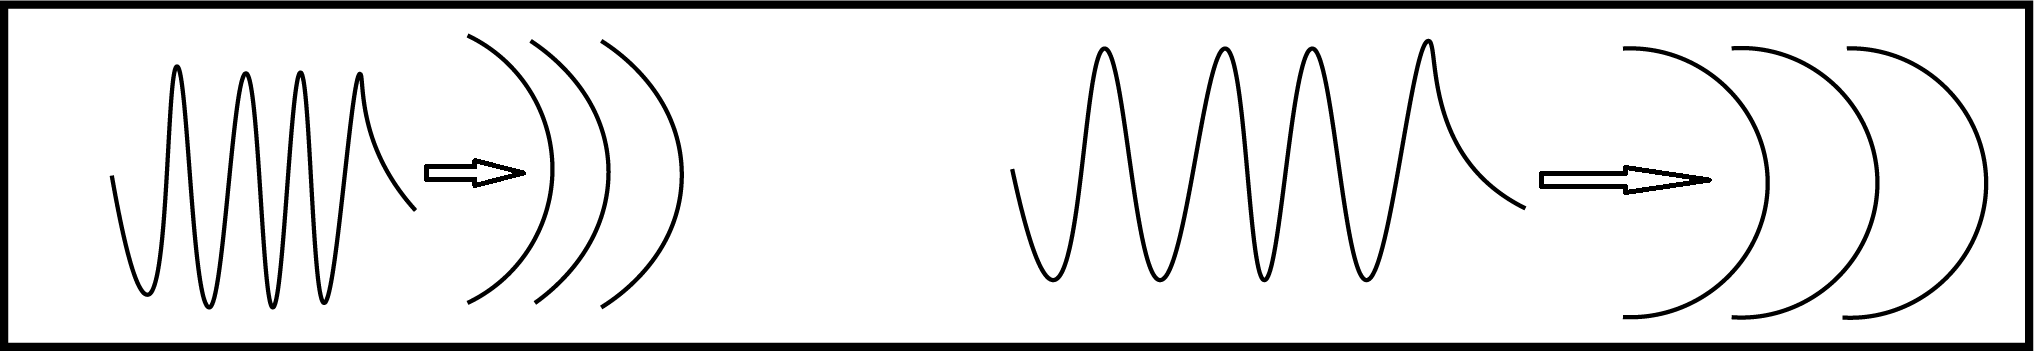
\includegraphics[width=0.8\textwidth]{Chapter1/lambwaves1.png}
    \caption{Lamb Waves Schematic \citep{rose2014ultrasonic}.}
    \label{fig:fig1}
\end{figure}

\begin{figure}[htbp]
    \centering
    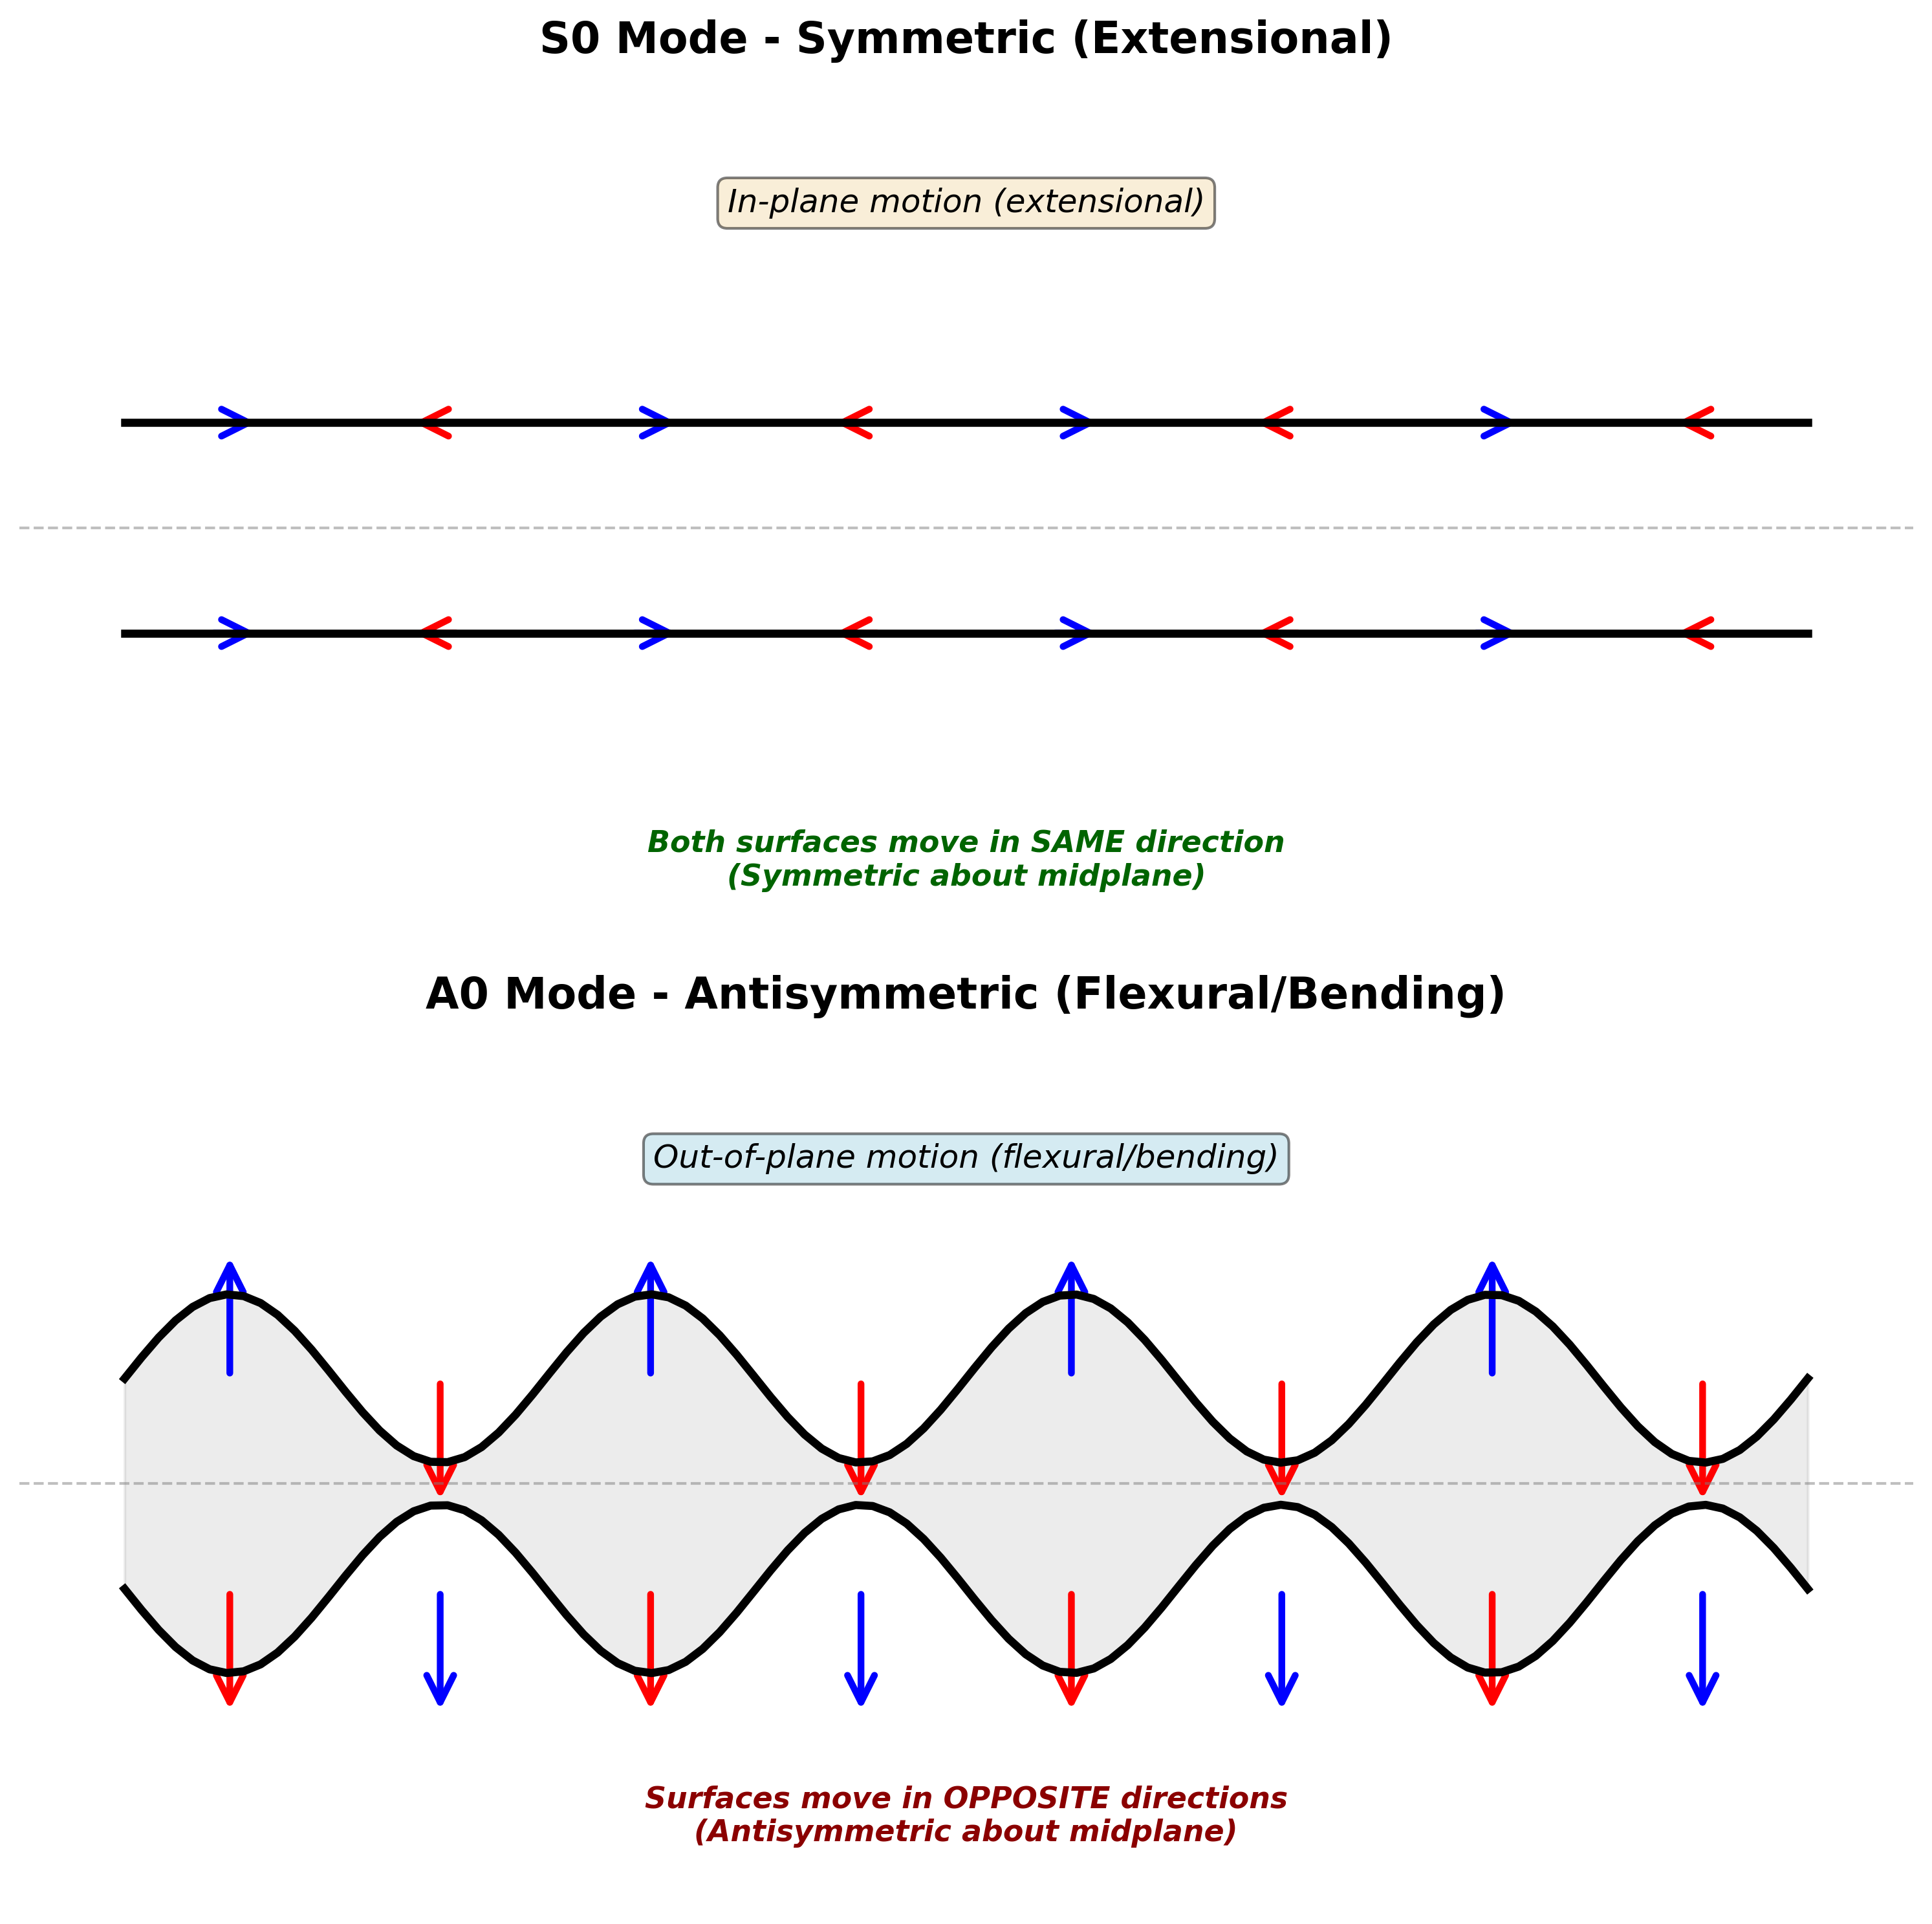
\includegraphics[width=0.8\textwidth]{Chapter1/A0_vs_S0_modes.png}
    \caption{Figure showing characteristics of symmetric and anti-symmetric wavemodes \citep{rose2014ultrasonic}.}
    \label{fig:S0andA0}
\end{figure}

\FloatBarrier   % forces both to appear before the next section text

These waves demonstrate remarkable versatility in damage detection capabilities. The waves exist in two fundamental types: symmetric modes (S0, S1, S2, ...) and antisymmetric modes (A0, A1, A2, ...) as shown in Figure~\ref{fig:S0andA0}, with them being most important because they carry more energy than higher-order modes \citep{GIURGIUTIU2014293}. Symmetric modes exhibit particle motion that is symmetric about the plate's midplane, with predominantly in-plane displacement resembling extensional motion. Antisymmetric modes display motion that is antisymmetric about the midplane, characterized by out-of-plane displacement similar to flexural or bending motion. Damage sensing with Lamb waves is based on the observation of alteration in the signal waveform due to changes in the propagation  \citep{Muller2017}. 



However, practical implementation faces significant challenges. Analysis of signals acquired by ultrasonic transducers can be cumbersome because of the overlapping of multiple dispersive wave modes and complex wave propagation due to scattering. The computational demands for accurate modeling become particularly intensive when solving inverse problems to characterize damage from measured responses, necessitating advanced numerical techniques and significant computational resources.

\section{Challenges in Lamb-Wave Modeling for Damage Detection}
\label{challenges}

Developing computational models for Lamb wave propagation presents a trade-off that always has to be addressed. The pursuit of accuracy, particularly for high-frequency waves traveling over extended distances through structures mingled with subtle defects, must be balanced against computational efficiency and the demands of real-time analysis.

The primary challenge is in selecting the most suitable modeling approaches. Two-dimensional finite element models excel at capturing the physics of wave propagation with exceptional detail. These models account for complex wave interactions, multiple mode conversions, and the subtle effects of structural discontinuities that one-dimensional approaches fundamentally cannot represent \citep{Fan2024}. However, this type of computational fidelity demands substantial resources. High-frequency content requires fine spatial and temporal discretization, resulting in simulation times that can span from hours to even days for a single analysis. Such computational requirements render 2D models impractical for the iterative processes inherent in damage detection applications.

One-dimensional models present an attractive alternative that operates orders of magnitude faster while providing reasonable approximations for certain wave propagation scenarios. Nevertheless, these simplified approaches sacrifice the important and complex physics that make Lamb waves particularly sensitive to structural changes. The resulting question becomes whether this sensitivity loss is acceptable when detecting potentially critical damage.

This computational dilemma intensifies when considering that damage detection inherently constitutes an inverse problem. Rather than executing a single simulation, the process requires hundreds or thousands of model evaluations as optimization algorithms search for damage parameters that best explain the measured data \citep{YU2023107030}. Each iteration demands a forward model evaluation (in our case), causing computational costs to accumulate rapidly. Or work with the mildly accurate 1D model, which would often give an incorrect estimation. These are referred to as Low-Fidelity Models (LFM). Engineers working with real structures often encounter an unavoidable constraint: they must employ high-fidelity 2D models (HFM) and wait for results over days, or accept the physical limitations of 1D LFM approximations, which carry the risk of missing critical damage indicators.

Surrogate modeling strategies emerge as a response to these limitations. Surrogate models are computationally inexpensive approximations constructed by training mathematical functions on datasets generated from physics-based simulations. Low-fidelity surrogates utilize simplified mathematical representations or reduced-order models, while multi-fidelity approaches combine information from multiple model types with varying computational costs and accuracies. Unlike high-fidelity models that solve governing equations directly, these surrogates employ techniques such as polynomial regression, neural networks, or Gaussian process regression to approximate complex physical relationships. The objective involves preserving the essential physics captured by 2D models while achieving computational efficiency that approaches or even surpasses the speeds of 1D approximations.

\section{Limitations of Single Fidelity Simulations and their Surrogates}
\label{Limitations of surrogates}

Single-fidelity surrogate models face challenges when high-fidelity physics-based simulations become computationally prohibitive. Constructing accurate surrogates requires sufficiently large training datasets from expensive simulations, which becomes impractical for computationally intensive problems where individual runs extend to several hours \citep{Giselle_Fern_ndez_Godino_2023} \citep{Wang2020}. The problem worsens when dealing with multiple input parameters. As the parameters increase, the amount of training data needed grows exponentially to maintain accuracy \citep{Jakeman2020}. For example, structural health monitoring applications involving Lamb wave propagation demand thousands of model evaluations, making single-fidelity approaches computationally unaffordable \citep{https://doi.org/10.1002/eqe.4116}. Conversely, constructing surrogates purely from low-fidelity models, while computationally attractive, risks substantial inaccuracy or distortion of system response when simplified models fail to capture critical phenomena such as nonlinear wave interactions \citep{ZHANG2022101430}.

To enable practical and scalable Structural Health Monitoring (SHM) frameworks, there is a need for an integrated multi-fidelity modeling approach that:
\begin{enumerate}
    \item Utilizes simplified beam-theory-based low-fidelity (LF) models to efficiently generate wave-response data,
    \item Retains the predictive precision of high-fidelity (HF) models through selective fusion of high-fidelity information, and
    \item Employs machine-learning-based surrogate modeling for rapid forward and inverse predictions across a range of damage scenarios.
\end{enumerate}

The central problem addressed in this thesis is therefore:

\medskip

\textbf{"To develop a computationally efficient, physics-consistent multi-fidelity surrogate modeling framework for accurate forward prediction and inverse identification of Lamb-wave responses in thin plate-like structures with surface-level damages."}

\section{Motivation and Research Gap}
\label{Research Gap}

Lamb waves have proven to be incredibly useful for detecting small damages in thin, plate-like structures, as we have established in the previous sections. These waves are particularly effective at detecting surface problems, making them ideal for monitoring the health of aerospace, naval, and mechanical components. However, there's a significant consideration when it comes to actually using and simulating these waves.
The primary challenge is striking a balance between accuracy and computational cost. When we want to capture Lamb wave behavior accurately, we need to account for high-frequency content and very fine geometric details. This means typically two-dimensional finite-element models with extremely refined meshes is needed. These high-fidelity models can accurately show how complex wave interactions and scattering happen when there's damage present. Unfortunately, they're computationally expensive to run. This makes it nearly impossible to conduct large-scale studies or perform inverse analyses in any reasonable timeframe.

To address computational costs, researchers turns to simplified one-dimensional beam-theory models. These offer huge computational advantages with fewer degrees of freedom while maintaining moderate accuracy. However, they fail to capture complex wave responses from defects and cannot properly model damage, such as notches, in order to achieve the accuracy needed for damage detection, thereby trading accuracy for speed. 

Refined Zigzag theory, originally proposed by Tessler et al. \citep{tessler2007refined}, emerged from a specific need to accurately model layered composite and sandwich structures. The zigzag approach utilizes piecewise linear functions that are superimposed on classical beam kinematics. This enables the theory to represent how displacement fields vary through the thickness of the structure, effectively bridging the gap between computationally efficient single-layer theories and expensive layer-wise approaches.
Recent advances in refined zigzag theory have demonstrated a potential for homogeneous beam applications. Tessler's 2015 work \citep{tessler2015refined} demonstrated that by minutely deviating the shear modulus of individual layers from their original value, homogeneous beams can achieve accuracy comparable to that of two-dimensional models. This layered approach, inherent in zigzag theory, also provides a distinct advantage for notch modeling, as the discrete layer representation enables a more accurate capture of stress concentrations and local deformation patterns around damage sites compared to conventional Euler-Bernoulli or Timoshenko theories. These two compelling features provide strong motivation for adopting the zigzag theory as the foundation for the low-fidelity modeling framework in this research.

Data-driven surrogate models offer another path forward for exploration and accelerating structural response prediction. These models learn from simulation data to rapidly emulate wave responses. However, there's an important limitation: surrogate models trained only on low-fidelity data tend to inherit the same inaccuracies present in the simplified underlying physics.
This limitation can be addressed through multi-fidelity learning frameworks, as we discussed earlier. These approaches combine information from both low and high-fidelity sources. They can deliver prediction accuracy that approaches full high-fidelity models while using only a fraction of the computational resources and time of even a low-fidelity model making both forward prediction and inverse damage identification practically feasible for real-world structural health monitoring applications.

\subsubsection{Research Gap}
Despite extensive studies on Lamb-wave modeling and machine-learning-based SHM, several limitations persist that hinder the practical deployment of these techniques in real-world structural monitoring applications:

\begin{enumerate}
    \item \textbf{Computational bottleneck:} While 2D finite element (FE) simulations are the best method for modeling Lamb waves, they are computationally expensive. This cost is driven by the need for very fine elements to accurately simulate high-frequency waves. As a result, extensive studies cannot be conducted to understand how different damage types and sensor placements affect wave behavior. This computational bottleneck slows down the development of effective structural health monitoring and damage detection systems \citep{WILLBERG2012246, SHEN2016116}.
    
    \item \textbf{Limited integration of physics and learning:} There aren't enough detailed studies comparing different beam theories to see how accurately they can model Lamb waves in structures with real-world damage. Timoshenko beam theory is generally more accurate than the simpler Euler-Bernoulli theory because it accounts for factors like shear and rotation, but because damage causes only very subtle changes in a wave's behavior and might occur mostly out of the midplane, thus becomes difficult to detect by 1D beam theory, choosing the most precise theory is crucial for actually detecting that damage. Most current research that compares these theories focuses on how waves disperse or spread out, rather than on how well the theories can be used to identify damage. This lack of research leaves us unsure which theoretical model is the most reliable and effective for practical engineering applications that use Lamb waves to find structural damage \citep{DIXIT20144341, LIMA1993449, JAIN2024118314}.
    \item \textbf{Limited integration of physics and learning:} Most machine learning (ML) models designed to analyze guided waves have a flaw: they are trained on limited, single-fidelity data, which causes them to make biased predictions and perform poorly when faced with new, unseen scenarios. While the underlying physics of these waves is complex to model directly, relying purely on ML creates another problem—these models are excellent at fitting the data they are trained on, but often fail disastarously when attempting to predict outcomes beyond their experience. The effectiveness of these data-driven models is also entirely dependent on the quality of the simulations used for training, meaning any errors in the initial simulation will compromise the model's ability to generalize to real-world experimental data. This gap between the ML approach and the fundamental physics of waves prevents the development of robust, "physics-aware" models that can reliably adapt to various damage scenarios and operating conditions \citep{Pawar2022, ROSAFALCO2021106604}.
    
    \item \textbf{Absence of efficient inverse formulations:} 
While forward simulations are studied widely, reliable damage localization and severity estimation using fast surrogate models remain underexplored. Inverse problems require the use of a model and the identification of uncertain parameters, where damage localization faces difficulties including modeling error, fidelity discrepancies and regularization challenges. Inverse damage identification using surrogates typically involves training models to map damage parameters to structural features, but existing approaches often struggle with accuracy limitations and capturing complex damage patterns. This constraint in model fidelity undermines the development of real-time damage assessment systems that require both computational efficiency and reliable predictions on intricate damage scenarios \citep{DadrasEslamlou2022, doi:10.1098/rsta.2006.1930}.
\end{enumerate}


This thesis addresses these gaps by developing and validating a multi-fidelity surrogate modeling framework that couples beam-theory simulations with machine-learning models to enable accurate and computationally efficient prediction and inference of Lamb-wave responses in damaged plates.

\section{Research Objectives}

This research aims to develop and validate a bi-fidelity surrogate modeling framework for structural response prediction in notched beam configurations and to apply this framework for efficient notch parameter identification in Lamb-wave-based SHM applications.


The specific objectives of this research are as follows:

\begin{enumerate}
    \item To investigate suitable low-fidelity physical models for Lamb-wave propagation in thin plate-like structures by comparing Euler--Bernoulli, Timoshenko, and zigzag beam theories under plane-strain conditions.
    
    \item To perform high-fidelity 2D finite-element simulations of a pitch--catch actuator--sensor configuration with surface-level rectangular notches representing different damage severities and locations.
    
    \item To construct a low-fidelity surrogate model (LFSM) using an autoencoder--XGBoost framework trained on 1D beam-model data for rapid forward prediction of wave responses.
    
    \item To develop a Bi-Fidelity Surrogate Model (BFSM) that fuses LFSM predictions with limited High Fidelity Model data to reduce modeling discrepancies and enhance predictive accuracy.
    
    \item To employ the BFSM for inverse damage identification, estimating the location and severity (stiffness-reduction category) of defects through an optimization-based approach.
    
    \item To evaluate the performance and generalization of the proposed framework across varying damage scenarios and material properties of linear-elastic metallic plates.
\end{enumerate}

\section{Organization of the Thesis}


This thesis is structured into seven chapters. Chapter 2 explains the physics of Lamb waves and how they propagate through structures. It covers the basic wave modes, dispersion behavior, and how waves scatter when they encounter damage. The chapter also discusses why simulating these waves is computationally challenging.

Chapter~3 describes how high fidelity simulation data is generated using 2D elastic beam theory. The numerical setup is detailed here, including governing equations, mesh design, boundary conditions, and how notches are modeled. This chapter also introduces different low-fidelity beam models and compares them against each other, particularly Euler--Bernoulli, Timoshenko, and zigzag beam theories.

The multi-fidelity modeling framework is presented in Chapter 4. It explains why combining different fidelity levels makes sense for structural health monitoring and reviews existing strategies like co-Kriging. The chapter then introduces the proposed framework and details how data from different sources is fused together. Training procedures and validation metrics are also covered.

Chapter 5 focuses on the machine learning methods used in this work. The autoencoder architecture is explained first, showing how it compresses wave response data into a compact representation. XGBoost is then introduced to model the relationship between damage parameters and these compressed features. The chapter demonstrates how these two components work together to form a complete prediction engine.

The practical application is demonstrated in Chapter 6 through a detailed case study. Different notch configurations are tested, and results from multi-fidelity and single-fidelity approaches are compared. The chapter evaluates both forward prediction accuracy and inverse problem notch parameters estimation. Physical interpretation of the results is emphasized throughout.

Chapter 7 concludes the thesis by summarizing key contributions and findings. Limitations of the current approach are discussed honestly, including assumptions about physics coverage and data requirements. Future research directions are suggested, such as experimental validation and integration with physics-informed neural networks.

\chapter{Fundamentals of Lamb Waves and its Role in SHM}

\section{Basics of Guided Ultrasonic Waves}

When mechanical disturbances propagate through infinite three-dimensional media, they travel as bulk waves—longitudinal waves that compress and extend the material, or shear waves that distort it transversally. Bulk waves are highly dispersive and dissipate easily as they propagate through the medium. However, when wave propagation occurs in structures with at least one dimension comparable to the wavelength, such as plates, shells, or beams, the wave behavior undergoes a fundamental change. The boundaries of the structure constrain the wave motion, giving rise to \textit{guided ultrasonic waves}. These waves are ``guided'' in the sense that they propagate along the structure while being confined by its geometry, repeatedly reflecting between the surfaces and creating characteristic wave patterns.

Unlike bulk waves that propagate in all directions and dissipate rapidly, guided waves can travel long distances along a structure with relatively low \citep{Yang2025Dataset}. This property enables a single transducer pair to interrogate large structural areas, making damage detection practical and cost-effective. In a typical SHM setup, an actuator generates a pulse that travels as a guided wave through the structure. Any discontinuity: a crack, delamination, or notch, causes partial reflection, mode conversion, and scattering of the incident wave. By analyzing the received signal at sensor locations, information about the damage can be extracted.

The mathematical description of guided waves begins with the equations of motion in an elastic medium. For a homogeneous, isotropic material, the displacement field $\mathbf{u}$ must satisfy the Navier-Cauchy equation:

\begin{equation}
\rho \frac{\partial^2 \mathbf{u}}{\partial t^2} = (\lambda + \mu) \nabla (\nabla \cdot \mathbf{u}) + \mu \nabla^2 \mathbf{u}
\end{equation}

where $\rho$ is the material density, and $\lambda$ and $\mu$ are the Lamé constants related to Young's modulus $E$ and Poisson's ratio $\nu$ through:

\begin{equation}
\lambda = \frac{E\nu}{(1+\nu)(1-2\nu)}, \quad \mu = \frac{E}{2(1+\nu)}
\end{equation}

For a structure with finite thickness, such as a plate of thickness $h$, traction-free boundary conditions must be imposed at the top and bottom surfaces. These conditions, combined with the equations of motion, yield a characteristic equation that results in discrete solutions. Each solution represents a distinct wave mode, characterized by its own displacement profile through the thickness and its own relationship between frequency and wave speed, a phenomenon known as \textit{dispersion} \citep{rose2014ultrasonic}.

\begin{figure}[h!]
\centering
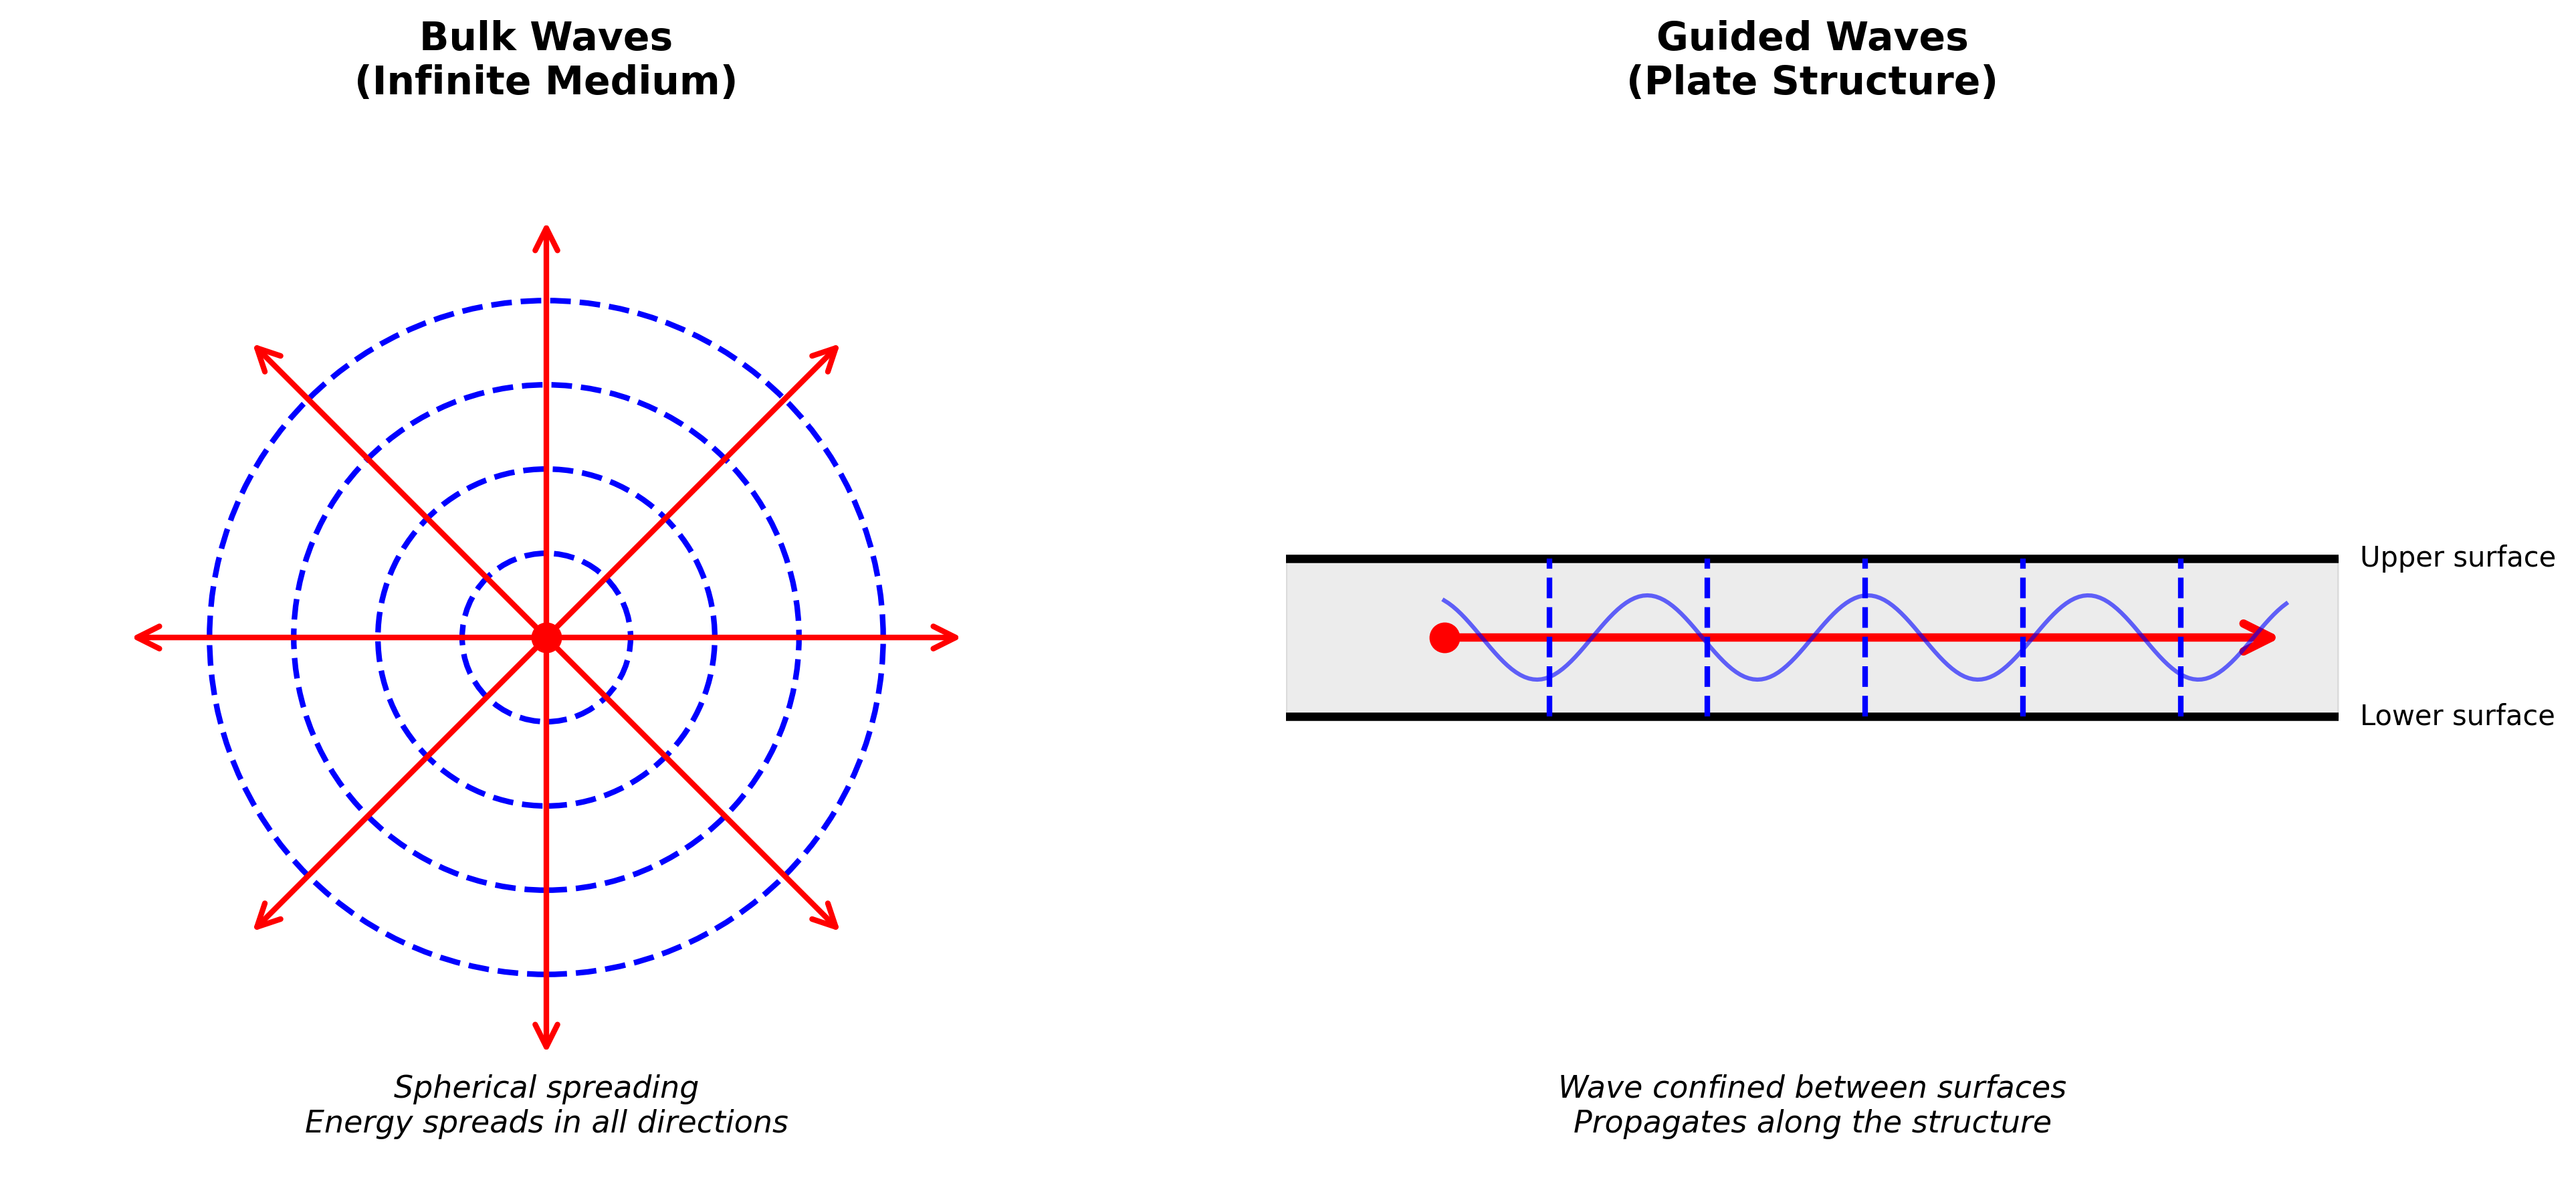
\includegraphics[width=1.0\textwidth]{Chapter2image/bulk_vs_guided_waves.png}
\caption{Schematic comparison of bulk waves vs guided waves}
\end{figure}

The energy carried by guided waves remains concentrated near the structure's surface, making them sensitive to surface-breaking defects and near-surface damage. Furthermore, because multiple modes can coexist at a given frequency, each with different velocity and displacement characteristics, careful selection of excitation frequency and mode allows tailoring the inspection to specific damage types and locations. This multimodal nature, while sometimes complicating signal interpretation, provides rich information about the structural condition when properly analyzed.

\section{Lamb Wave Modes (S\textsubscript{0} and A\textsubscript{0}'s Dispersion Behavior)}

Lamb waves, named after Horace Lamb who first derived their mathematical description in 1917, are a specific class of guided ultrasonic waves that propagate in thin plates or plate-like structures. Unlike surface waves such as Rayleigh waves that decay exponentially with depth, Lamb waves involve the entire thickness of the plate. They exist because the stress-free boundary conditions at both surfaces create standing wave patterns through the thickness, while the wave propagates freely along the plate.

The fundamental characteristic that distinguishes different Lamb wave modes is the symmetry of their displacement field with respect to the plate's midplane. Symmetric modes, denoted by $S$ with a numerical subscript ($S_0, S_1, S_2, \ldots$), exhibit displacement profiles that are symmetric about the midplane, refer Figure \ref{fig:S0andA0}. In the fundamental symmetric mode $S_0$, particles on the top and bottom surfaces move in phase with each other. The through-thickness displacement pattern resembles extensional motion at low frequencies, with particles moving predominantly parallel to the propagation direction. Antisymmetric modes, denoted by $A$ with subscripts ($A_0, A_1, A_2, \ldots$), have displacement profiles that are antisymmetric about the midplane. The fundamental antisymmetric mode $A_0$ features out-of-phase motion between top and bottom surfaces refer Figure \ref{fig:S0andA0}, producing a flexural or bending-like deformation, especially at low frequencies.

The mathematical treatment begins with assuming harmonic wave solutions of the form:

\begin{equation}
\mathbf{u}(x, z, t) = \mathbf{U}(z)e^{i(kx - \omega t)}
\end{equation}

where $x$ is the propagation direction, $z$ is the through-thickness coordinate, $k$ is the wavenumber, and $\omega$ is the angular frequency. Substituting this into the governing equations and applying traction-free boundary conditions at $z = \pm h/2$ yields the Rayleigh-Lamb frequency equations. For symmetric modes:

\begin{equation}
\frac{\tan(\beta h/2)}{\tan(\alpha h/2)} = -\frac{4k^2 \alpha \beta}{(k^2 - \beta^2)^2}
\end{equation}

For antisymmetric modes:

\begin{equation}
\frac{\tan(\beta h/2)}{\tan(\alpha h/2)} = -\frac{(k^2 - \beta^2)^2}{4k^2 \alpha \beta}
\end{equation}

where $\alpha$ and $\beta$ are related to the wavenumber and material properties through:

\begin{equation}
\alpha^2 = \frac{\omega^2}{c_L^2} - k^2, \quad \beta^2 = \frac{\omega^2}{c_T^2} - k^2
\end{equation}

with $c_L = \sqrt{(\lambda + 2\mu)/\rho}$ being the longitudinal wave speed and $c_T = \sqrt{\mu/\rho}$ the shear wave speed \citep{SU2016353}.

These transcendental equations have no closed-form solutions and must be solved numerically for each frequency. Each solution corresponds to a mode with a specific wavenumber $k$, from which the phase velocity $c_p = \omega/k$ and group velocity $c_g = d\omega/dk$ can be determined. The resulting dispersion curves—plots of phase velocity or group velocity versus frequency—are fundamental to understanding Lamb wave behavior.


The dispersion behavior has profound implications for SHM applications. At low frequency-thickness products (typically $fd < 1$~MHz$\cdot$mm, where $f$ is frequency and $d$ is thickness), only the fundamental modes $S_0$ and $A_0$ propagate. The $S_0$ mode approaches the plate wave velocity at very low frequencies, exhibiting minimal dispersion, while the $A_0$ mode is highly dispersive, with its velocity approaching zero as frequency decreases. This means that an $A_0$ wavepacket will spread out significantly as it propagates, with higher frequency components traveling faster than lower frequencies.

The choice between $S_0$ and $A_0$ modes for damage detection involves tradeoffs. The $S_0$ mode's lower dispersion and higher velocity enable cleaner signals and faster inspection, making it favorable for large-area scanning. However, the $A_0$ mode's flexural nature makes it more sensitive to surface-breaking defects, delaminations, and thickness variations. In practice, excitation typically generates both modes simultaneously, and the resulting signal contains contributions from each mode arriving at different times due to their different group velocities. This multimodal nature can be exploited—by analyzing arrival times and amplitude changes of individual modes, more comprehensive damage characterization becomes possible than with single-mode analysis alone.

The computational challenge in predicting Lamb wave interactions with damage stems directly from this dispersion behavior. Time-domain finite element simulations must resolve multiple wavelengths with sufficient spatial discretization while tracking wave evolution over distances many times the plate thickness. The frequency-dependent velocities mean that narrow-band excitation produces relatively simple waveforms, while broadband pulses—often preferred for time-domain resolution—create complex, dispersive signals that require sophisticated post-processing. This computational burden motivates the development of surrogate models and multi-fidelity approaches, where expensive high-fidelity simulations are complemented by faster, approximate models, enabling rapid damage detection and characterization.

\section{Wave Propagation and Scattering Due to Defects}

The utility of Lamb waves for structural health monitoring relies on their interaction with structural discontinuities. When a propagating wave encounters damage—whether a crack, notch, delamination, or corrosion—the local change in geometry and material properties disrupts the wavefield. This disruption manifests as a combination of reflection, transmission, mode conversion, and scattering, each carrying information about the defect's characteristics \citep{rose2014ultrasonic,ahn2021lamb}. Understanding these interaction mechanisms is essential for interpreting measured signals and extracting damage parameters.

Consider a Lamb wave propagating along a structure and encountering a notch or through-thickness defect. The incident wave can be decomposed into symmetric and antisymmetric components, each with its own wavenumber and displacement profile. At the defect location, the stress-free boundary condition within the damage region cannot be satisfied by the incident wave alone. The wavefield must adjust to accommodate this new boundary, generating reflected and transmitted waves that travel away from the defect. The principle of superposition requires that the total displacement field—incident plus scattered waves—satisfies both the governing equations throughout the domain and the boundary conditions at all surfaces, including those created by the damage \citep{ahn2021lamb}.

The scattering process is inherently multimodal. Even if a pure $S_0$ mode impinges on a defect, the scattered field generally contains both $S_0$ and $A_0$ components, along with higher-order modes if the excitation frequency permits their propagation. This phenomenon, known as \textit{mode conversion}, occurs because the defect breaks the symmetry that would otherwise preserve modal purity \citep{ahn2021lamb}. A symmetric defect placed exactly at the plate midplane produces less mode conversion than an asymmetric defect or one located off-center, but some conversion typically occurs due to the complex three-dimensional stress redistribution around the damage \citep{cawley2018practical}.

The amplitude of reflected and transmitted waves depends on the defect's size relative to the wavelength. For damage dimensions much smaller than the wavelength, the defect acts as a point scatterer, with energy radiating in multiple directions but relatively weak reflection in the backward direction. As the defect size approaches or exceeds the wavelength, specular reflection becomes significant, and the scattered field develops directional characteristics \citep{rose2014ultrasonic}. This frequency-dependent interaction means that damage of a given size will interact more strongly with higher-frequency components of a broadband pulse, while lower frequencies may pass with minimal disturbance.

Quantitatively, the scattered wavefield can be expressed through the concept of \textit{scattering coefficients} \citep{ahn2021lamb}. For a defect at position $x_d$, the total displacement field can be written as:

\begin{equation}
u_{\text{total}}(x,z,t) = u_{\text{incident}}(x,z,t) + 
\sum_{m} R_m \, u_m^{\text{reflected}}(x,z,t) + 
\sum_{n} T_n \, u_n^{\text{transmitted}}(x,z,t)
\end{equation}

where the summations run over all propagating modes, and $R_m$ and $T_n$ are the reflection and transmission coefficients for modes $m$ and $n$, respectively. These coefficients are complex-valued, encoding both amplitude and phase changes. For a given incident mode and defect geometry, these coefficients can be determined through analytical methods for simple geometries or, more commonly, through numerical simulation for realistic damage scenarios \citep{ahn2021lamb,rose2014ultrasonic}.

The spatial distribution of the scattered field exhibits characteristic patterns. Directly behind the defect (in the forward direction), a shadow zone may form where the transmitted wave amplitude is reduced \citep{Im}. This amplitude reduction provides a direct measure of damage severity when sensors are positioned on opposite sides of the defect \citep{na2021review}. In the backward direction, the reflected wave interferes with the incident wave, creating standing wave patterns near the defect that contain information about the defect location through the phase relationship between incident and reflected components \citep{rose2014ultrasonic}.

\begin{figure}[h]
\centering
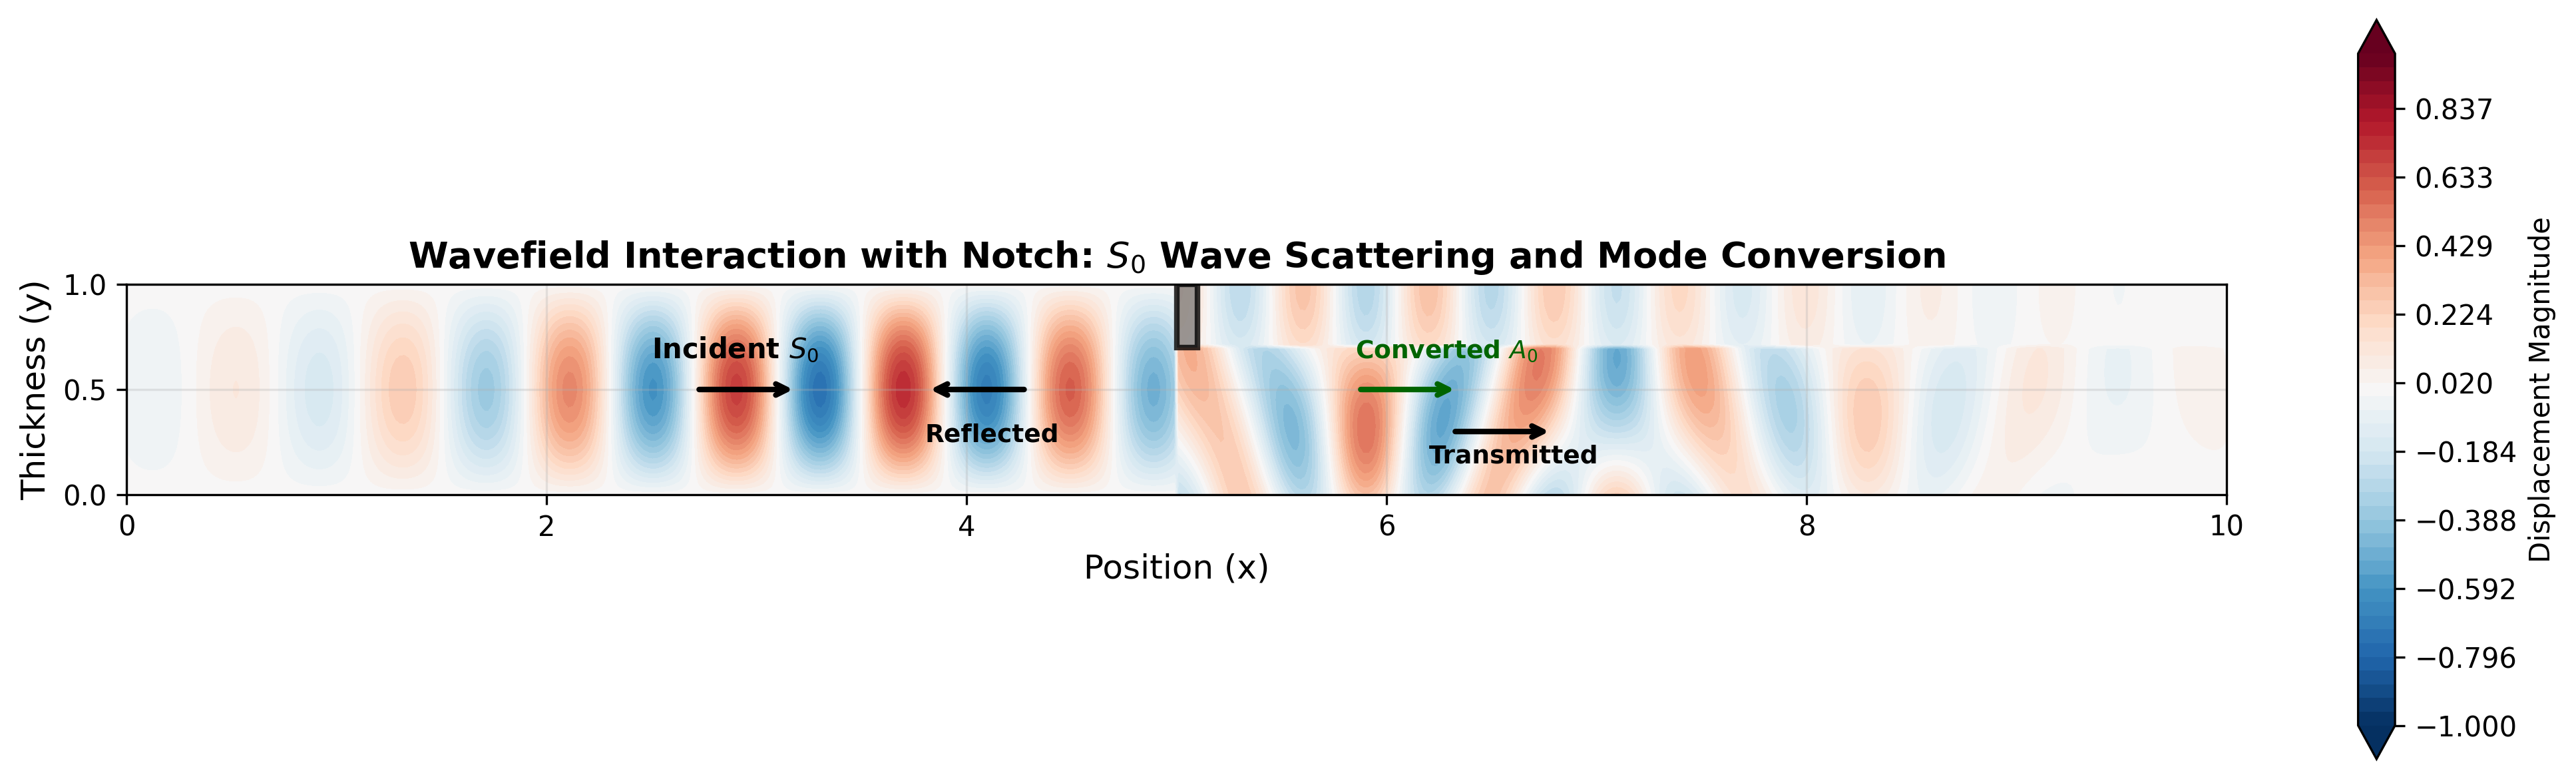
\includegraphics[width=1\textwidth]{Chapter2image/wavefield_notch.png}
\caption{Snapshot of wavefield interaction with a notch showing incident $S_0$ wave from left, reflected wave packet traveling backward, transmitted wave with reduced amplitude continuing forward, and mode-converted $A_0$ component propagating with different velocity. Color contours show displacement magnitude and arrows indicate wave fronts \citep{article}.}
\label{fig:wave_scattering}
\end{figure}

For notch-type defects, which are common in fatigue damage and manufacturing flaws, the scattering mechanism involves both the sharp geometric discontinuity at the notch edges and the reduced load-carrying capacity within the notch region. The notch creates a local flexibility, causing the structure to deform more readily under the incident wave's stress field. This enhanced deformation radiates secondary waves that comprise the scattered field. Deeper notches produce stronger scattering because they represent more significant impedance changes; wider notches scatter more energy because they interact with the wave over a larger spatial extent \citep{cawley2018practical, KIM2011734}.

The temporal characteristics of scattered signals are equally important. When a transient pulse encounters damage, the reflected signal arrives back at the source location after a time delay determined by the damage location and the wave velocity \citep{rose2014ultrasonic}. If both $S_0$ and $A_0$ modes are present, each will have different arrival times due to their different group velocities, creating multiple reflection peaks in the time-domain signal. The temporal separation between these peaks provides complementary information about the defect location, enabling cross-validation and improving robustness against measurement uncertainties and mode identification errors \citep{na2021review}.

\section{Use of Lamb Waves in Damage Detection}

Lamb wave-based damage detection involves generating waves through piezoelectric transducers, allowing propagation through the structure to interact with damage, and measuring the resulting wavefield at sensor locations~\cite{giurgiutiu2005}. Comparing measurements with baseline data, physics-based model predictions or surrogate model predictions enables inference of damage presence, location, and characteristics.

Pulse-echo testing uses a transducer to generate a pulse that reflects from damage, returning after time delay $\Delta t$. The damage location $x_d$ relative to transducer position $x_0$ is:
\begin{equation}
x_d = x_0 + \frac{c_g \cdot \Delta t}{2}
\end{equation}
where $c_g$ is the group velocity and the factor of two accounts for round-trip travel. Multiple modes generate multiple reflection peaks, providing redundant distance measurements.

Pitch-catch configurations use separated actuator-sensor pairs~\cite{su2009}. Damage between transducers causes three signal changes: amplitude reduction in the direct path, additional scattered wave arrivals at intermediate times, and mode conversion introducing new modal components. The received signal is:
\begin{equation}
u_{\text{measured}}(x_s, t) = u_{\text{direct}}(x_s, t) + \sum_{i} u_{\text{scattered}}^{(i)}(x_s, t) + n(t)
\end{equation}
where $u_{\text{direct}}$ is the undamaged response, the sum represents scattering from all damage sites, and $n(t)$ is noise.

Triangulation using multiple transducer pairs enables localization~\cite{giurgiutiu2008}. Three or more pitch-catch measurements detecting the same defect create intersecting elliptical loci pinpointing damage location. Accuracy depends on transducer network density, time-of-flight precision, and velocity accuracy.

Damage characterization extracts quantitative defect information. Signal features correlating with damage include scattered wave amplitude (increasing with defect size), frequency content changes (larger defects scatter lower frequencies), and time-domain waveform shape (encoding defect geometry).


Integration of Lamb wave measurements with machine learning and surrogate modeling addresses traditional challenges. Data-driven models learn complex relationships directly from data, bypassing analytical scattering solutions. The multi-fidelity framework combines expensive high-fidelity simulations with abundant low-fidelity data, enabling the characterization of damage for real-world monitoring. The following chapters develop these concepts, showing how computational and machine learning tools transform Lamb wave measurements into precise, quantitative damage assessments.

\chapter{Simulation of Lamb Waves using 2D Elastic Beam and Reduced Order Model Theories}
\label{Introduce different 1D models and a reference 2D model}

The generation of multi-fidelity datasets requires a clear understanding of the underlying theoretical frameworks that produce low- and high-fidelity simulations. This chapter begins with a detailed exposition of zigzag theory, a refined approach for modeling composite structures that accounts for layer-wise material discontinuities. The theory is then compared with classical one-dimensional models, such as Timoshenko and Euler-Bernoulli, to establish its computational advantages for wave propagation problems. Following this, the two-dimensional elastic beam theory is introduced as the high-fidelity reference model, which provides ground truth solutions by solving the full elasticity equations without kinematic assumptions. The chapter concludes by describing the systematic generation of both low- and high-fidelity datasets and their validation through wavefield visualization. The distinction between these fidelity levels lies not in the choice of software but in the fundamental theoretical assumptions that govern each approach.

%%%%%%%%%%%%%%%%%%%%%%%%%%%%%%%%%%%%%%%%%%%%%%%%%%%%%%%%%%%%%%%%%%%%%%%%%%%%%%%%%%%%%%%%%%%%%%%%%%%%%%%%%%%%%%%%%%%%%%%%%%%%%%%%%%%%%%%%%%%%%%%%%%%%%%%%%%%%%%%%%%%%%

\section{1D Beam Zigzag Theory}
\label{sec:zigzag_theory}
The zigzag theory for laminated composite beams represents a refinement of classical beam theories that addresses the limitations of traditional approaches when dealing with layered structures. We first develop this theory for a general composite case where material properties vary across layers. Unlike classical theories that assume linear displacement variation through the beam thickness, zigzag theory incorporates the material discontinuities between layers by allowing piecewise-linear displacement patterns that capture the sudden changes in material properties at layer interfaces. Subsequently, we examine the limiting case of a homogeneous beam to establish the use case for our research in relation to established classical results.

Consider a laminated composite beam of total height $h$ consisting of $N$ perfectly bonded layers, where each layer $k$ extends from coordinate $z_{k-1}$ to $z_k$ measured from a reference plane. The beam extends along the longitudinal $x$-direction with length $L$, while the $z$-direction represents the through-thickness coordinate. The fundamental assumption underlying zigzag theory is that the axial displacement exhibits a layerwise linear variation that accounts for the transverse shear deformation effects neglected in classical beam theories.

The theory assumes that each layer behaves as a linear elastic material with distinct material properties, creating interfaces where material properties change discontinuously. These material discontinuities generate interlaminar shear stress concentrations that classical theories cannot accurately predict. The zigzag approach addresses this limitation by introducing a zigzag function that captures the layer-dependent linear variation of axial displacement while maintaining displacement continuity across layer interfaces.

For the specific case of three-layer composite beams under consideration, the layers are designated as bottom ($k=1$), middle ($k=2$), and top ($k=3$), with interfaces located at $z_1$ and $z_2$. Each layer possesses distinct elastic moduli $E^{(k)}$, shear moduli $G^{(k)}$, and densities $\rho^{(k)}$, while maintaining perfect bonding at all interfaces.

The displacement field in zigzag theory is expressed through three primary kinematic variables that represent the global beam behavior, enhanced by a zigzag function that captures local layer effects. The axial displacement $u(x,z,t)$ is formulated as:

\begin{equation}
    u(x,z,t) = u_0(x,t) - z \frac{\partial w_0}{\partial x}(x,t) + R^{(k)}(z) \, \psi_0(x,t)
\end{equation}


where \(u_0(x,t)\) represents the axial displacement of the reference plane located at \(z = 0\), \(w_0(x,t)\) denotes the transverse displacement, and \(\psi_0(x,t)\) is the shear deformation parameter related to the average shear strain of the reference plane. The term \(- z \frac{\partial w_0}{\partial x}\)

represents the classical Euler--Bernoulli contribution, while $R^{(k)}(z)$ is the layer-dependent zigzag function.

The transverse displacement is assumed to remain constant across the beam thickness, consistent with the assumption of inextensible normals:
\begin{equation}
   w(x,z,t) = w_0(x,t) 
\end{equation}


This assumption is valid for slender beams where the length-to-thickness ratio is sufficiently large, typically greater than $10$. For the analysis of ultrasonic wave propagation in composite beams, this assumption remains appropriate given the high frequency content and the associated short wavelengths relative to beam thickness.

The displacement field can be expressed in compact matrix form as:

\begin{equation}
\mathbf{u}(x,z,t) = 
\begin{Bmatrix}
u(x,z,t) \\
w(x,z,t)
\end{Bmatrix}
=
\begin{bmatrix}
1 & -z\frac{\partial }{\partial x} & R^{(k)}(z) \\
0 & 1 & 0
\end{bmatrix}
\begin{Bmatrix}
u_0(x,t) \\
w_0(x,t) \\
\psi_0(x,t)
\end{Bmatrix}
\end{equation}


This formulation reduces the infinite degrees of freedom associated with the continuum displacement field to three generalized displacement variables, enabling efficient computational implementation while maintaining the essential physics of layered beam behavior.

\begin{figure}[htbp]
\centering
\includegraphics[width=\textwidth]{zigzaglayer.png}
\caption{Schematic Representation of an
N-Layer Laminated Composite Beam}
\label{fig:zigzag_layer}
\end{figure}

The strain components relevant to beam theory are the axial strain $\varepsilon_x$ and the transverse shear strain $\gamma_{xz}$. These strains are derived from the displacement field through standard kinematic relations.

The axial strain is obtained as:
\begin{equation}
\varepsilon_x = \frac{\partial u}{\partial x} 
= \frac{\partial u_0}{\partial x} 
- z \frac{\partial^2 w_0}{\partial x^2} 
+ R^{(k)}(z) \frac{\partial \psi_0}{\partial x}
\end{equation}

This expression reveals the three distinct contributions to axial strain: the membrane strain 
$\frac{\partial u_0}{\partial x}$, the bending strain 
$- z \frac{\partial^2 w_0}{\partial x^2}$, and the zigzag contribution 
$R^{(k)}(z) \frac{\partial \psi_0}{\partial x}$ that captures the layer-wise linear variation.

The transverse shear strain is formulated as:
\begin{equation}
\gamma_{xz} = \frac{\partial u}{\partial z} + \frac{\partial w}{\partial x} 
= \frac{\partial R^{(k)}}{\partial z} \, \psi_0 
\end{equation}

Since the transverse displacement is independent of $z$, the shear strain depends only on the derivative of the zigzag function. The term 
$\frac{\partial R^{(k)}}{\partial z}$ represents the layer-wise constant shear strain within each layer, while maintaining the necessary discontinuities at layer interfaces to accommodate different material properties.

The strain field can be expressed in matrix notation as:
\begin{equation}
\begin{Bmatrix} \varepsilon_x \\ \gamma_{xz} \end{Bmatrix} =
\begin{bmatrix} 
\frac{\partial}{\partial x} & -z \frac{\partial^2}{\partial x^2} & R^{(k)}(z) \frac{\partial}{\partial x} \\
0 & 0 & \frac{\partial R^{(k)}}{\partial z} 
\end{bmatrix}
\begin{Bmatrix} u_0 \\ w_0 \\ \psi_0 \end{Bmatrix}
\end{equation}


The zigzag function $R^{(k)}(z)$ must satisfy several critical conditions to ensure physical consistency and mathematical well-posedness. These conditions include displacement continuity at layer interfaces, stress continuity requirements, and appropriate boundary conditions at the beam's top and bottom surfaces.

For a three-layer beam, the zigzag function is constructed as a piecewise cubic polynomial within each layer:
\begin{equation}
R^{(k)}(z) = a_0^{(k)} + a_1^{(k)} z + a_2^{(k)} z^2 + a_3^{(k)} z^3
\end{equation}

where the coefficients $a_0^{(k)}$, $a_1^{(k)}$, $a_2^{(k)}$, and $a_3^{(k)}$ are determined through the enforcement of continuity and boundary conditions.

The fundamental continuity conditions require that the axial displacement remains continuous across layer interfaces. At the interface between layers $k$ and $k+1$ located at $z = z_k$, this condition yields:
\begin{equation}
R^{(k)}(z_k) = R^{(k+1)}(z_k)
\end{equation}

Additionally, the transverse shear stress must remain continuous across interfaces to maintain equilibrium. This condition is expressed as:
\begin{equation}
G^{(k)} \gamma_{xz}^{(k)} = G^{(k+1)} \gamma_{xz}^{(k+1)} \quad \text{at} \quad z = z_k
\end{equation}

Substituting the shear strain expression, this becomes:
\begin{equation}
G^{(k)} \frac{\partial R^{(k)}}{\partial z}\bigg|_{z=z_k} = 
G^{(k+1)} \frac{\partial R^{(k+1)}}{\partial z}\bigg|_{z=z_k}
\end{equation}

The boundary conditions at the top and bottom surfaces require that the transverse shear stress vanishes for a free surface:
\begin{equation}
\gamma_{xz}^{(1)}\bigg|_{z=z_0} = \frac{\partial R^{(1)}}{\partial z}\bigg|_{z=z_0} \, \psi_0 = 0
\end{equation}

\begin{equation}
\gamma_{xz}^{(N)}\bigg|_{z=z_N} = \frac{\partial R^{(N)}}{\partial z}\bigg|_{z=z_N} \, \psi_0 = 0
\end{equation}

The determination of the zigzag function coefficients requires establishing a system of twelve equations to uniquely define the twelve unknown coefficients. This system incorporates displacement continuity conditions at layer interfaces, shear stress continuity requirements, boundary conditions at free surfaces, and appropriate normalization constraints.
The systematic solution of this constraint system yields the explicit expressions for the zigzag function coefficients in each layer. These coefficients define the piecewise cubic polynomials that capture the layer-wise linear variation of axial displacement while maintaining all necessary continuity and equilibrium requirements. The resulting zigzag functions completely characterize the enhanced displacement field and enable accurate representation of the through-thickness shear deformation behavior in laminated composite beams.



\subsection{Constitutive Relations for Composite Layers}

The constitutive relations for each layer relate the stress components to the strain components through the material properties. For each layer $k$, assuming isotropic material behavior within the layer, the stress-strain relations are:

\begin{align}
\sigma_x^{(k)} &= E^{(k)} \, \varepsilon_x^{(k)} \\
\tau_{xz}^{(k)} &= G^{(k)} \, \gamma_{xz}^{(k)}
\end{align}



where $E^{(k)}$ and $G^{(k)}$ are the elastic and shear moduli of layer $k$, respectively. For isotropic materials, the shear modulus is related to the elastic modulus through:

\begin{equation}
G^{(k)} = \frac{E^{(k)}}{2 \left( 1 + \nu^{(k)} \right)}
\end{equation}


where $\nu^{(k)}$ is Poisson's ratio for layer $k$.

Substituting the strain expressions into the constitutive relations yields:

\begin{equation}
\sigma_x^{(k)} = E^{(k)} \left[ 
\frac{\partial u_0}{\partial x} 
- z \frac{\partial^2 w_0}{\partial x^2} 
+ R^{(k)}(z) \frac{\partial \psi_0}{\partial x} 
\right]
\end{equation}


\begin{equation}
\tau_{xz}^{(k)} = G^{(k)} \left[ 
\frac{\partial R^{(k)}}{\partial z} \, \psi_0 
\right]
\end{equation}


These expressions reveal how the zigzag theory naturally captures the layer-wise variation of stresses while maintaining the necessary continuity conditions at interfaces.

\subsection{Variational formulation and governing equations}
\label{sec:variational}


The governing equations for the zigzag beam theory are derived using Hamilton's principle, which states that the motion of a dynamic system between two specified times makes the action integral stationary. For conservative systems, Hamilton's principle is formulated as:

\begin{equation}
\delta \int_{t_1}^{t_2} L \, dt = 0
\end{equation}

where the Lagrangian is given by
\begin{equation}
L = T - U
\end{equation}
representing the difference between the kinetic energy $T$ and the strain energy $U$. The variational operator $\delta$ denotes the first variation of the action integral with respect to the generalized coordinates.

\subsection*{Kinetic Energy Formulation}

The kinetic energy for a three-layer zigzag beam of length $L$ and width $b$ is expressed as:

\begin{equation}
T = \frac{1}{2} \int_0^L \int_{z_0}^{z_3} \rho^{(k)} 
\left[ \left(\frac{\partial u}{\partial t}\right)^2 
     + \left(\frac{\partial w}{\partial t}\right)^2 \right] 
\, b \, dz \, dx
\end{equation}

where $\rho^{(k)}$ denotes the density of layer $k$.  
Substituting the zigzag displacement field expressions:

\begin{align}
u(x,z,t) &= u_0(x,t) - z \frac{\partial w_0}{\partial x}(x,t) 
           + R^{(k)}(z) \, \psi_0(x,t) \\[6pt]
w(x,z,t) &= w_0(x,t)
\end{align}

and performing the through-thickness integration yields:

\begin{align}
T = \frac{1}{2} \int_0^L \Big[ & I_{00}\dot{u}_0^2 + I_{00}\dot{w}_0^2 
+ I_{11}\left(\frac{\partial \dot{w}_0}{\partial x}\right)^2 + I_{22}\dot{\psi}_0^2 \nonumber \\
& - 2I_{01}\dot{u}_0\frac{\partial \dot{w}_0}{\partial x} 
+ 2I_{02}\dot{u}_0\dot{\psi}_0 
- 2I_{12}\frac{\partial \dot{w}_0}{\partial x}\dot{\psi}_0 \Big] dx
\end{align}


The inertia coefficients are defined through layerwise integration:

\begin{align}
I_{00} &= \sum_{k=1}^{3} \rho^{(k)} b \int_{z_{k-1}}^{z_k} dz 
       = \sum_{k=1}^{3} \rho^{(k)} b \, h^{(k)} \\[6pt]
I_{01} &= \sum_{k=1}^{3} \rho^{(k)} b \int_{z_{k-1}}^{z_k} z \, dz \\[6pt]
I_{02} &= \sum_{k=1}^{3} \rho^{(k)} b \int_{z_{k-1}}^{z_k} R^{(k)}(z) \, dz \\[6pt]
I_{11} &= \sum_{k=1}^{3} \rho^{(k)} b \int_{z_{k-1}}^{z_k} z^2 \, dz \\[6pt]
I_{12} &= \sum_{k=1}^{3} \rho^{(k)} b \int_{z_{k-1}}^{z_k} z \, R^{(k)}(z) \, dz \\[6pt]
I_{22} &= \sum_{k=1}^{3} \rho^{(k)} b \int_{z_{k-1}}^{z_k} \left[ R^{(k)}(z) \right]^2 dz
\end{align}
where 
\begin{equation}
h^{(k)} = z_k - z_{k-1}
\end{equation}
represents the thickness of layer $k$.

\subsection*{Strain Energy Formulation}

The strain energy is expressed in terms of the stress and strain components:

\begin{equation}
U = \frac{1}{2} \int_0^L \int_{z_0}^{z_3} 
\left( \sigma_x^{(k)} \, \varepsilon_x^{(k)} 
     + \tau_{xz}^{(k)} \, \gamma_{xz}^{(k)} \right) 
b \, dz \, dx
\end{equation}

Substituting the constitutive relations and strain expressions, and performing the through-thickness integration yields:

\begin{align}
U = \frac{1}{2} \int_0^L &\Bigg[ 
A_{11} \left(\frac{\partial u_0}{\partial x}\right)^2 
+ A_{22} \left(\frac{\partial^2 w_0}{\partial x^2}\right)^2 
+ A_{33} \left(\frac{\partial \psi_0}{\partial x}\right)^2 
+ A_{44} \, \psi_0^2 \nonumber \\[6pt]
&- 2A_{12} \frac{\partial u_0}{\partial x} \frac{\partial^2 w_0}{\partial x^2} 
+ 2A_{13} \frac{\partial u_0}{\partial x} \frac{\partial \psi_0}{\partial x} 
- 2A_{23} \frac{\partial^2 w_0}{\partial x^2} \frac{\partial \psi_0}{\partial x}
\Bigg] dx
\end{align}

The stiffness coefficients are defined as:

\begin{align}
A_{11} &= \sum_{k=1}^{3} E^{(k)} b \int_{z_{k-1}}^{z_k} dz \\[6pt]
A_{12} &= \sum_{k=1}^{3} E^{(k)} b \int_{z_{k-1}}^{z_k} z \, dz \\[6pt]
A_{13} &= \sum_{k=1}^{3} E^{(k)} b \int_{z_{k-1}}^{z_k} R^{(k)}(z) \, dz \\[6pt]
A_{22} &= \sum_{k=1}^{3} E^{(k)} b \int_{z_{k-1}}^{z_k} z^2 \, dz \\[6pt]
A_{23} &= \sum_{k=1}^{3} E^{(k)} b \int_{z_{k-1}}^{z_k} z \, R^{(k)}(z) \, dz \\[6pt]
A_{33} &= \sum_{k=1}^{3} E^{(k)} b \int_{z_{k-1}}^{z_k} \left[R^{(k)}(z)\right]^2 dz \\[6pt]
A_{44} &= \sum_{k=1}^{3} G^{(k)} b \int_{z_{k-1}}^{z_k} \left[ \frac{\partial R^{(k)}}{\partial z} \right]^2 dz
\end{align}


\subsection*{Derivation of Governing Equations}

Application of Hamilton's principle to the Lagrangian $L = T - U$ requires:

\begin{equation}
\delta \int_{t_1}^{t_2} (T - U) \, dt = 0
\end{equation}

Taking variations with respect to each generalized coordinate and applying integration by parts yields the three coupled governing equations:

\paragraph{Axial Force Equilibrium:}
\begin{equation}
\frac{\partial N}{\partial x} 
= I_{11} \frac{\partial^2 u_0}{\partial t^2} 
- I_{12} \frac{\partial^2}{\partial x \, \partial t^2} w_0 
+ I_{13} \frac{\partial^2 \psi_0}{\partial t^2}
\end{equation}

\paragraph{Transverse Force and Moment Equilibrium:}
\begin{equation}
\frac{\partial^2 M}{\partial x^2} + \frac{\partial V_x}{\partial x} 
= -I_{12} \frac{\partial^2}{\partial x \, \partial t^2} u_0 
+ I_{22} \frac{\partial^2}{\partial x^2 \partial t^2} w_0 
- I_{23} \frac{\partial^2}{\partial x \, \partial t^2} \psi_0
\end{equation}

\paragraph{Zigzag Shear Equilibrium:}
\begin{equation}
\frac{\partial P}{\partial x} - V_x 
= I_{13} \frac{\partial^2 u_0}{\partial t^2} 
- I_{23} \frac{\partial^2}{\partial x \, \partial t^2} w_0 
+ I_{33} \frac{\partial^2 \psi_0}{\partial t^2}
\end{equation}

\subsection*{Stress Resultant Definitions}

The stress resultants are defined through through-thickness integration of stresses:

\paragraph{Axial Force Resultant:}
\begin{align}
N &= \sum_{k=1}^{3} \int_{z_{k-1}}^{z_k} \sigma_x^{(k)} b \, dz \nonumber \\
  &= A_{11} \frac{\partial u_0}{\partial x} 
   - A_{12} \frac{\partial^2 w_0}{\partial x^2} 
   + A_{13} \frac{\partial \psi_0}{\partial x}
\end{align}

\paragraph{Bending Moment Resultant:}
\begin{align}
M &= \sum_{k=1}^{3} \int_{z_{k-1}}^{z_k} \sigma_x^{(k)} z \, b \, dz \nonumber \\
  &= A_{12} \frac{\partial u_0}{\partial x} 
   - A_{22} \frac{\partial^2 w_0}{\partial x^2} 
   + A_{23} \frac{\partial \psi_0}{\partial x}
\end{align}

\paragraph{Zigzag Stress Resultant:}
\begin{align}
P &= \sum_{k=1}^{3} \int_{z_{k-1}}^{z_k} \sigma_x^{(k)} R^{(k)}(z) b \, dz \nonumber \\
  &= A_{13} \frac{\partial u_0}{\partial x} 
   - A_{23} \frac{\partial^2 w_0}{\partial x^2} 
   + A_{33} \frac{\partial \psi_0}{\partial x}
\end{align}

\paragraph{Transverse Shear Force Resultant:}
\begin{align}
V_x &= \sum_{k=1}^{3} \int_{z_{k-1}}^{z_k} \tau_{xz}^{(k)} b \, dz \nonumber \\
    &= B_{1} \frac{\partial w_0}{\partial x} + B_{2} \, \psi_0
\end{align}
where $B_{1} = \langle Q_{55} \rangle$ and $B_{2} = \langle Q_{55} \, R^{(k)}_{,z} \rangle$ are effective shear coefficients obtained from through-thickness integration.

\subsection*{Boundary Conditions}

The natural boundary conditions derived from the variational principle are:  
At any boundary ($x = 0$ or $x = L$), either the displacement or the corresponding force resultant must be specified:

\[
u_0 \; \text{specified} \quad \text{or} \quad N = 0
\]

\[
w_0 \; \text{specified} \quad \text{or} \quad V_x = 0
\]

\[
\frac{\partial w_0}{\partial x} \; \text{specified} \quad \text{or} \quad M = 0
\]

\[
\psi_0 \; \text{specified} \quad \text{or} \quad P = 0
\]

These governing equations and boundary conditions completely characterize the dynamic behavior of three-layer zigzag beams. The theory captures the essential physics of layered structures through the zigzag displacement field while maintaining computational efficiency through the use of only three generalized displacement variables. The coupling between axial, bending, and zigzag effects through the inertia terms enables accurate prediction of wave propagation phenomena in laminated composite beams.

\subsection{Finite Element Implementation of Zigzag Theory}

The finite element method provides a systematic approach for discretizing the continuous zigzag beam theory into a computationally tractable form. The implementation requires careful consideration of interpolation functions, element formulation, and assembly procedures to maintain theoretical accuracy while ensuring numerical stability.



\subsubsection*{Element Formulation and Interpolation Functions}

The zigzag beam is discretized using two-node beam elements with enhanced kinematics. Each element contains physical nodes at its ends, and the nodal degrees of freedom are selected to ensure compatibility with the governing equations and continuity requirements.

At each node $i$, the degrees of freedom are defined as:
\begin{equation}
    \mathbf{q}_i = \begin{Bmatrix} u_{0i} \\ w_{0i} \\ \theta_i \\ \psi_{0i} \end{Bmatrix}
\end{equation}

where $u_{0i}$ and $w_{0i}$ are the axial and transverse displacements, $\theta_i$ is the rotation of the transverse normal, and $\psi_{0i}$ is the zigzag amplitude.

The complete element displacement vector is:
\begin{equation}
    \mathbf{q}^e = \begin{Bmatrix} u_{01} \\ w_{01} \\ \theta_1 \\ \psi_{01} \\ u_{02} \\ w_{02} \\ \theta_2 \\ \psi_{02} \end{Bmatrix}.
\end{equation}


Linear Lagrange interpolation is employed for $u_0$ and $\psi_0$, while cubic Hermite interpolation is used for $w_0$ to ensure $C^1$ continuity. The interpolation functions are expressed in matrix form as:
\begin{equation}
   \begin{Bmatrix} u_0(\xi) \\ w_0(\xi) \\ \psi_0(\xi) \end{Bmatrix} 
= \mathbf{N}(\xi) \, \mathbf{q}^e,
\end{equation}

where $\mathbf{N}(\xi)$ is the shape function matrix and $\xi$ is the natural coordinate.

\begin{figure}[htbp]
\centering
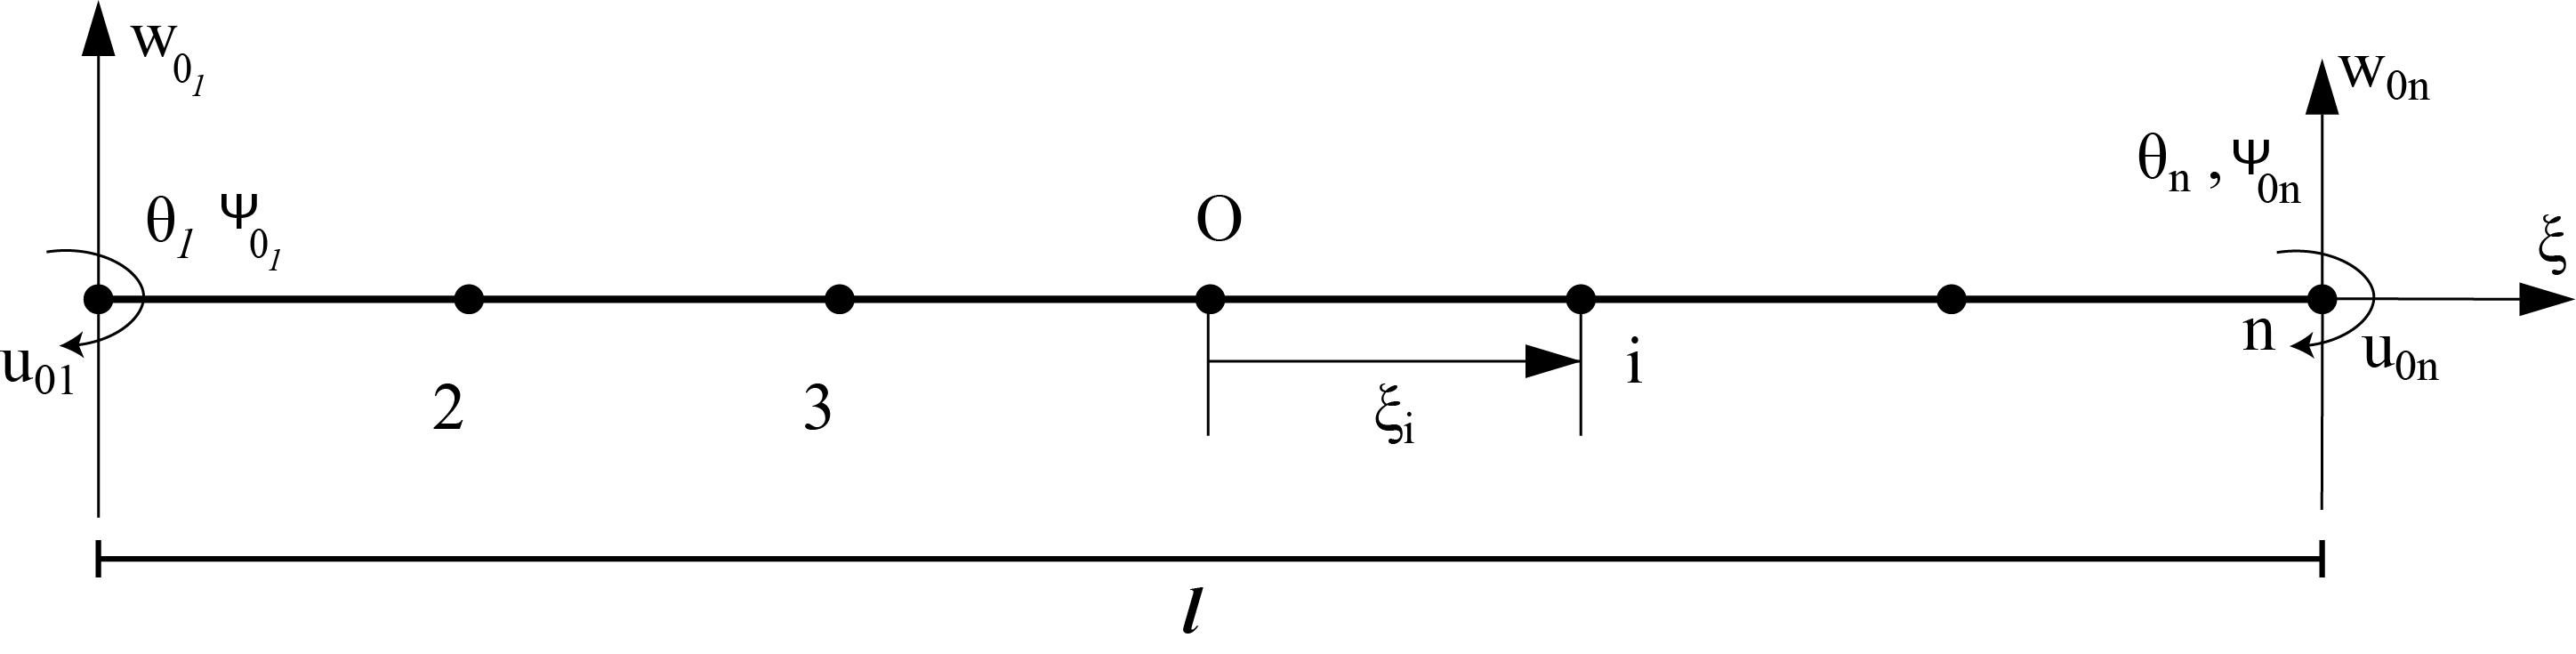
\includegraphics[width=\textwidth]{coordinate_system.png}
\caption{A spectral strip element, formulated using zigzag theory (ZIGT), which possesses 'n' internal nodes, each with associated degrees of freedom (DOFs)}
\label{fig:coordinate_system}
\end{figure}

\subsection*{Strain-Displacement Matrix Formulation}

The strain-displacement relationships are derived by differentiating the interpolation functions. The axial and transverse shear strains are given by:
\begin{equation}
    \varepsilon_x = \frac{\partial u_0}{\partial x} - z \frac{\partial^2 w_0}{\partial x^2} + R^{(k)}(z)\frac{\partial \psi_0}{\partial x}
\end{equation}

\begin{equation}
    \gamma_{xz} = \frac{\partial R^{(k)}}{\partial z} \psi_0 
\end{equation}


These relations are expressed in terms of nodal displacements through the strain-displacement matrix $\mathbf{B}^{(k)}$ for layer $k$.

\subsubsection*{Element Mass Matrix}

The element mass matrix is derived from the kinetic energy expression, which involves velocity products of the interpolated displacement field. The general form is:
\begin{equation}
    \mathbf{M}^e = \int_{-1}^{+1} \sum_{k=1}^{N} \int_{z_{k-1}}^{z_k} 
\rho^{(k)} \left[ \mathbf{N}_u^T \mathbf{N}_u + \mathbf{N}_w^T \mathbf{N}_w \right] b \, \frac{l_e}{2} \, dz \, d\xi,
\end{equation}

where $\rho^{(k)}$ is the density of layer $k$, and $\mathbf{N}_u$, $\mathbf{N}_w$ are the submatrices of $\mathbf{N}$ associated with axial and transverse displacements.

\subsubsection*{Element Stiffness Matrix}

The element stiffness matrix is obtained from the strain energy:
\begin{equation}
    \mathbf{K}^e = \int_{-1}^{+1} \sum_{k=1}^{N} \int_{z_{k-1}}^{z_k} 
(\mathbf{B}^{(k)})^T \mathbf{D}^{(k)} \mathbf{B}^{(k)} \, b \, \frac{l_e}{2} \, dz \, d\xi
\end{equation}

where $\mathbf{D}^{(k)}$ is the constitutive matrix of layer $k$. The layerwise zigzag function $R^{(k)}(z)$ and its derivative introduce coupling terms that enrich the kinematics of the beam element.

\subsubsection*{Numerical Integration and Assembly}

Numerical integration is employed due to the complexity of the integrands involving the zigzag function and material heterogeneity. Gaussian quadrature is applied in both the in-plane and through-thickness directions, with integration performed separately within each layer. The global mass and stiffness matrices are assembled from the element contributions, yielding the system:
\begin{equation}
\mathbf{M} \ddot{\mathbf{Q}} + \mathbf{C} \dot{\mathbf{Q}} + \mathbf{K} \mathbf{Q} = \mathbf{F}(t),
\end{equation}
where $\mathbf{Q}$ is the global displacement vector.

%%%%%%%%%%%%%%%%%%%%%%%%%%%%%%%%%%%%%%%%%%%%%%%%%%%%%%%%%%%%%%%%%%%%%%%%%%%%%%%%%%%%%%%%%%%%%%%%%%%%%%%%%%%%%%%%%%%

\section{Comparative Analysis of One-Dimensional Beam Theories for Lamb Wave Propagation}
\label{sec:comparison_1d_theories}

Having established the theoretical foundation of zigzag beam theory in the previous section, it becomes essential to evaluate its performance relative to classical one-dimensional beam theories. This comparison serves two purposes: first, it validates the necessity of employing a refined theory for Lamb wave propagation analysis; second, it demonstrates why zigzag theory constitutes an appropriate choice for the low-fidelity model in the multi-fidelity framework. This section introduces the classical Euler--Bernoulli and Timoshenko beam theories, establishes a numerical benchmark problem involving a notched beam, and presents a comparative analysis of wave propagation responses predicted by the three theories.

\subsection{Classical One-Dimensional Beam Theories}

\subsubsection{Euler--Bernoulli Beam Theory}

The Euler--Bernoulli beam theory represents the simplest framework for analyzing beam deformation and has been extensively employed in structural dynamics for over two centuries. The theory rests on the fundamental kinematic assumption that plane sections initially perpendicular to the beam axis remain plane and perpendicular after deformation. This assumption implicitly neglects transverse shear deformation, making the theory most accurate for slender beams where the length-to-height ratio exceeds approximately 10.

The displacement field in Euler--Bernoulli theory is expressed as:
\begin{equation}
u(x,z,t) = u_0(x,t) - z \frac{\partial w_0}{\partial x}(x,t), \quad w(x,z,t) = w_0(x,t)
\end{equation}
where $u_0$ and $w_0$ represent the axial and transverse displacements of the beam axis, respectively. The governing equations for free vibration, derived from Hamilton's principle, reduce to two uncoupled partial differential equations:

\begin{align}
EA \frac{\partial^2 u_0}{\partial x^2} &= \rho A \frac{\partial^2 u_0}{\partial t^2} \label{eq:EB_axial}\\
EI \frac{\partial^4 w_0}{\partial x^4} + \rho A \frac{\partial^2 w_0}{\partial t^2} &= 0 \label{eq:EB_bending}
\end{align}

where $A$ is the cross-sectional area and $I$ is the second moment of area. The first equation governs longitudinal wave propagation with wave speed $c_L = \sqrt{E/\rho}$, while the second describes flexural wave propagation. The flexural waves exhibit strong dispersion, with the dispersion relation $\omega^2 = EI k^4 / (\rho A)$, where $k$ is the wavenumber.

The theory's principal limitation for high-frequency wave propagation stems from its neglect of shear deformation and rotary inertia. For Lamb wave frequencies typically employed in structural health monitoring (50--500 kHz), these effects become significant, particularly for the antisymmetric mode $A_0$, which possesses strong flexural characteristics.

\subsubsection{Timoshenko Beam Theory}

Timoshenko beam theory addresses the primary deficiency of Euler--Bernoulli theory by incorporating transverse shear deformation and rotary inertia effects. The theory introduces an independent rotation variable $\phi(x,t)$ that is no longer constrained to equal the slope of the deflected axis $\partial w_0/\partial x$. The difference between these quantities represents the shear deformation of the beam.

The displacement field in Timoshenko theory takes the form:
\begin{equation}
u(x,z,t) = u_0(x,t) - z \phi(x,t), \quad w(x,z,t) = w_0(x,t)
\end{equation}

The governing equations for the transverse motion consist of two coupled partial differential equations:
\begin{align}
\kappa GA \left(\frac{\partial w_0}{\partial x} - \phi\right) &= \rho A \frac{\partial^2 w_0}{\partial t^2} \label{eq:Tim_shear}\\
EI \frac{\partial^2 \phi}{\partial x^2} + \kappa GA \left(\frac{\partial w_0}{\partial x} - \phi\right) &= \rho I \frac{\partial^2 \phi}{\partial t^2} \label{eq:Tim_moment}
\end{align}

where $\kappa$ is the shear correction factor, typically taken as $5/6$ for rectangular cross-sections, which accounts for the non-uniform distribution of shear stress across the beam height. The longitudinal motion remains governed by Eq.~\eqref{eq:EB_axial}.

Timoshenko theory provides improved accuracy for moderately thick beams and extends the valid frequency range compared to Euler--Bernoulli theory. However, the constant shear correction factor represents an approximation that cannot capture the true through-thickness variation of displacement and stress fields. Furthermore, for layered or damaged structures where material properties vary through the thickness, the single-valued shear correction factor becomes inadequate.

\subsubsection{Comparison with Zigzag Theory}

Table~\ref{tab:theory_comparison} presents a systematic comparison of the three beam theories. The zigzag theory distinguishes itself through its ability to represent piecewise-linear through-thickness displacement variation via the zigzag function $R^{(k)}(z)$. This capability proves essential for accurately capturing Lamb wave behavior, where different wave modes exhibit distinct through-thickness displacement patterns.

\begin{table}[h]
\centering
\caption{Comparison of one-dimensional beam theories}
\label{tab:theory_comparison}
\begin{tabular}{lccc}
\toprule
\textbf{Feature} & \textbf{Euler--Bernoulli} & \textbf{Timoshenko} & \textbf{Zigzag} \\
\midrule
DOFs per node & 2 & 3 & 4 \\
Through-thickness variation & Linear & Linear & Piecewise cubic \\
Shear deformation & Neglected & Constant & Layer-wise \\
Rotary inertia & Neglected & Included & Included \\
Suitable for high-freq. waves & Poor & Moderate & Good \\
Computational cost (relative) & 1$\times$ & 1.5$\times$ & \approx 1.5$\times$ \\
\bottomrule
\end{tabular}
\end{table}

The computational cost of zigzag theory, while higher than classical theories due to the additional degree of freedom, remains orders of magnitude lower than two-dimensional finite element analysis. This favorable balance between accuracy and computational efficiency motivates its selection as the low-fidelity model for the multi-fidelity surrogate framework.

\subsection{Numerical Benchmark Configuration}

To quantitatively assess the predictive capabilities of the three beam theories, a benchmark problem is established involving Lamb wave propagation in a notched aluminum beam. The configuration is designed to represent a realistic structural health monitoring scenario where a pitch-catch transducer pair interrogates a structure containing surface damage.

\subsubsection{Beam Geometry and Material Properties}

The benchmark beam possesses the following geometric and material characteristics:

\begin{itemize}
    \item \textbf{Length:} $L = 3.0$ m
    \item \textbf{Height:} $h = 1.5$ mm
    \item \textbf{Width:} $b = 1.0$ m (plane strain conditions)
    \item \textbf{Material:} Aluminum
    \item \textbf{Young's modulus:} $E = 70$ GPa
    \item \textbf{Density:} $\rho = 2700$ kg/m$^3$
    \item \textbf{Poisson's ratio:} $\nu = 0.33$
\end{itemize}

These dimensions yield a length-to-height ratio of 2000, representing a thin plate-like structure typical of aerospace and mechanical components. The material properties correspond to aluminum alloy 6061, commonly employed in structural applications due to its favorable strength-to-weight ratio and corrosion resistance.

\subsubsection{Notch Configuration}

A rectangular notch is introduced to simulate surface damage resulting from fatigue crack initiation, corrosion, or manufacturing defects. The notch parameters are:

\begin{itemize}
    \item \textbf{Location:} $x_{\text{notch}} = 1.75$ m
    \item \textbf{Depth:} $d_{\text{notch}} = 1.0$ mm (67\% of beam height)
    \item \textbf{Width:} $w_{\text{notch}} = 1.0$ mm
\end{itemize}

The notch depth of 1.0 mm represents significant structural damage, reducing the local height to 0.5 mm. This substantial reduction in cross-section creates pronounced wave scattering and mode conversion effects, providing a stringent test for the beam theories' ability to capture damage-induced wave phenomena.

Figure~\ref{fig:benchmark_geometry} shows the general setup for the current benchmark configuration and serves as the basis for further tests to be discussed in the following sections.

\begin{figure}[h]
\centering
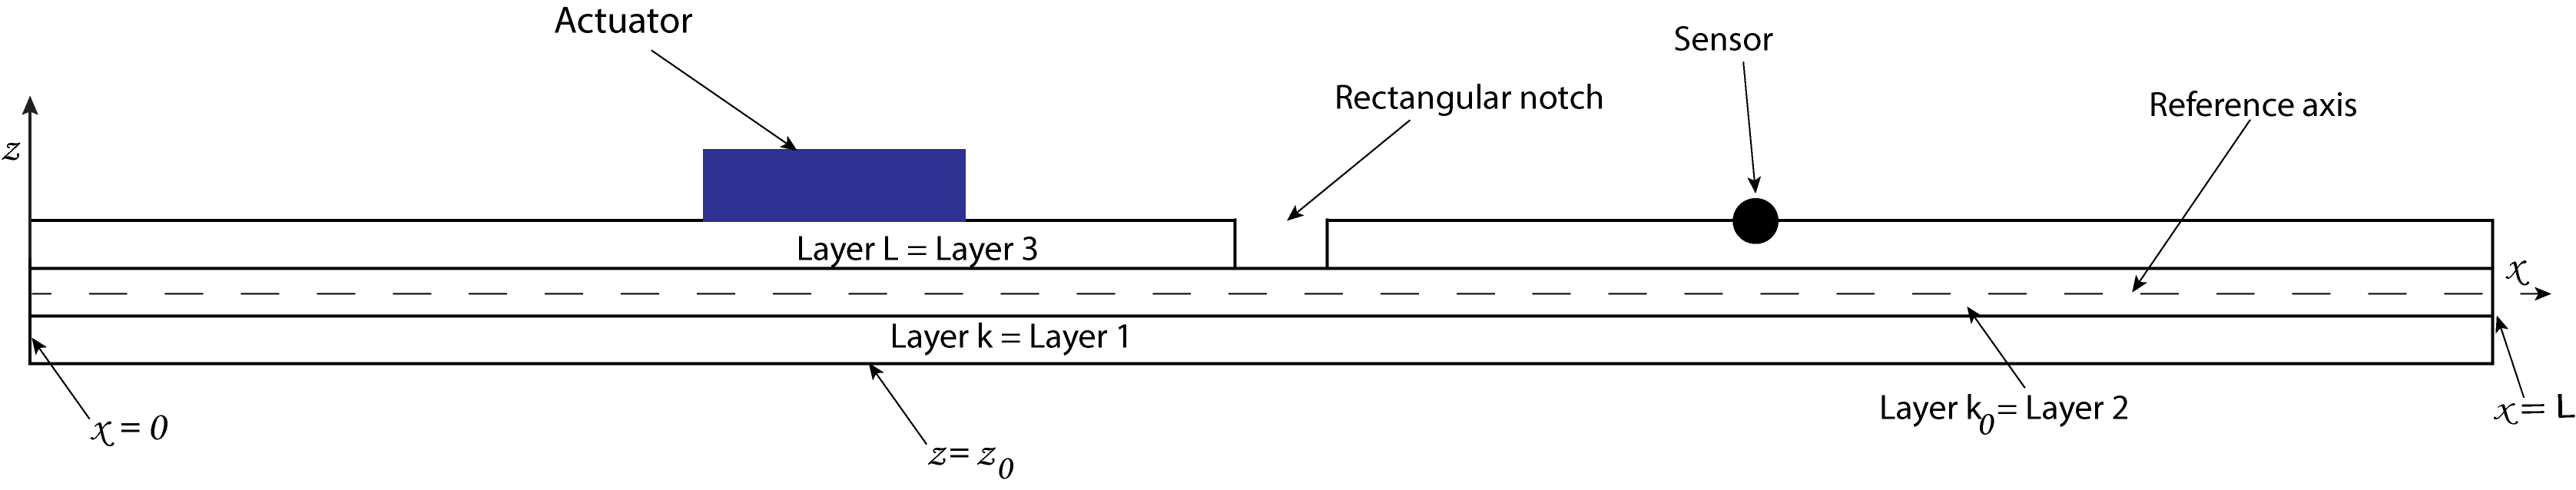
\includegraphics[width=\textwidth]{beamgeometry.png}
\caption{General setup of the benchmark beam configuration with notch, actuator positions, and sensor location.}
\label{fig:benchmark_geometry}
\end{figure}

\subsubsection{Actuator-Sensor Configuration}

The analysis employs a pitch-catch configuration, where an actuator generate a pulse wave that propagates toward the notch, with a sensor positioned beyond the notch to capture transmitted and scattered waves. The specific configuration is:

\textbf{Actuators:}
\begin{itemize}
    \item Actuator edge 1: $x_1 = 1.6465$ m
    \item Actuator edge 2: $x_2 = 1.6535$ m
    \item Separation distance: $\Delta x = 7.0$ mm
    \item Actuation mode: Differential (out-of-phase)
\end{itemize}

The actuators apply equal magnitude but opposite sign forces, creating a localized bending moment. This differential actuation preferentially excites the antisymmetric $A_0$ mode while minimizing the symmetric $S_0$ mode, though both modes are present in the response due to the finite actuator separation and structural boundary conditions.

\textbf{Sensor:}
\begin{itemize}
    \item Position: $x_{\text{sensor}} = 1.95$ m
    \item Through-thickness location: $z_{\text{sensor}} = 0.75$ mm (top surface)
    \item Distance from notch: 0.20 m
    \item Measured quantity: Axial displacement $u(x_{\text{sensor}}, z_{\text{sensor}}, t)$
\end{itemize}

The sensor location at the top surface enables detection of both symmetric and antisymmetric modes, as well as any mode-converted waves generated by the notch. The 200 mm distance from the notch provides sufficient separation to resolve distinct wave packets for the incident, reflected, and transmitted waves.

\subsubsection{Excitation Signal}

The excitation force follows a Hanning-windowed toneburst signal, commonly employed in ultrasonic testing to provide a compromise between time-domain localization and frequency content:

\begin{equation}
F(t) = \begin{cases}
A_0 \left[1 - \cos\left(\frac{2\pi t}{T_{\text{active}}}\right)\right] \sin(2\pi f_c t) & 0 \leq t \leq T_{\text{active}} \\
0 & t > T_{\text{active}}
\end{cases}
\end{equation}

where:
\begin{itemize}
    \item $A_0$ = Amplitude (normalized to unity for comparison)
    \item $f_c$ = 100 kHz (center frequency)
    \item $T_{\text{active}}$ = 50 $\mu$s (active excitation duration)
    \item Total observation time: $T_{\text{total}}$ = 300 $\mu$s
\end{itemize}

The 100 kHz center frequency is selected based on typical structural health monitoring practice, providing a wavelength on the order of 50 mm for the $S_0$ mode, which is sufficiently long for wave propagation over meter-scale distances while remaining sensitive to millimeter-scale damage features. The Hanning window ensures smooth onset and termination of the excitation, minimizing unwanted high-frequency spectral content.

Figure~\ref{fig:excitation_signal} displays the time-domain excitation signal, illustrating the Hanning envelope and the 100 kHz carrier frequency.

\begin{figure}[h]
\centering
\fbox{\parbox{0.9\textwidth}{\centering\vspace{4cm}PLACEHOLDER FIGURE\\Excitation signal showing:\\- Hanning window envelope (dashed line)\\- 100 kHz sinusoidal carrier\\- Active duration: 0--50 $\mu$s\\- Time axis: 0--300 $\mu$s\\\vspace{4cm}}}
\caption{Hanning-windowed toneburst excitation signal at 100 kHz center frequency.}
\label{fig:excitation_signal}
\end{figure}

\subsection{Notch Modeling in Classical Theories}

A fundamental challenge in applying classical beam theories to damaged structures concerns the representation of geometric discontinuities such as notches, cracks, or holes. Unlike zigzag theory, which can accommodate spatially-varying layer properties and through-thickness geometry changes, Euler--Bernoulli and Timoshenko theories require alternative approaches to model localized damage.

\subsubsection{Stiffness Reduction Approach}

In the present analysis, the notch is modeled in classical theories through local reduction of the beam's extensional and bending stiffnesses. For a rectangular notch extending from the top surface to depth $d_{\text{notch}}$, the reduced cross-sectional properties in the notched region are:

\textbf{Reduced height:}
\begin{equation}
h_{\text{reduced}} = h - d_{\text{notch}} = 1.5 - 1.0 = 0.5 \text{ mm}
\end{equation}

\textbf{Reduced cross-sectional area:}
\begin{equation}
A_{\text{reduced}} = b \cdot h_{\text{reduced}} = 1.0 \times 0.5 = 0.5 \times 10^{-3} \text{ m}^2
\end{equation}

This represents a 67\% reduction in cross-sectional area compared to the undamaged region.

\textbf{Reduced second moment of area:}
\begin{equation}
I_{\text{reduced}} = \frac{b h_{\text{reduced}}^3}{12} = \frac{1.0 \times (0.5 \times 10^{-3})^3}{12} = 1.04 \times 10^{-11} \text{ m}^4
\end{equation}

The second moment of area experiences a more dramatic reduction of 92\% relative to the undamaged section, as it scales with the cube of the height. Consequently, the notch creates a substantially more compliant region for bending deformation than for axial deformation.

In the finite element implementation, elements located within the notch region ($x_{\text{notch}} - w_{\text{notch}}/2 \leq x \leq x_{\text{notch}} + w_{\text{notch}}/2$) are assigned the reduced stiffness values:
\begin{align}
(EA)_{\text{notch}} &= E \cdot A_{\text{reduced}} = 70 \times 10^9 \times 0.5 \times 10^{-3} = 3.5 \times 10^7 \text{ N} \\
(EI)_{\text{notch}} &= E \cdot I_{\text{reduced}} = 70 \times 10^9 \times 1.04 \times 10^{-11} = 7.3 \times 10^{-1} \text{ N·m}^2
\end{align}

\subsubsection{Limitations of the Stiffness Reduction Approach}

While computationally straightforward, the stiffness reduction method possesses several fundamental limitations that compromise its accuracy for wave propagation analysis:

\begin{enumerate}
    \item \textbf{Smeared damage representation:} The approach distributes the notch's effect over the element length, failing to capture the sharp geometric discontinuity at the notch edges. In reality, stress concentrations occur at these edges, generating localized wave scattering that cannot be represented by a smooth stiffness variation.

    \item \textbf{Neglect of through-thickness effects:} The reduction in cross-sectional properties is calculated assuming the neutral axis shifts to the mid-height of the reduced section. However, the true stress and displacement distributions near the notch exhibit complex three-dimensional patterns that single-valued stiffness parameters cannot capture.

    \item \textbf{Inadequate mode conversion modeling:} When a Lamb wave encounters a notch, the geometric asymmetry induces mode conversion between symmetric and antisymmetric modes. The stiffness reduction approach cannot represent this phenomenon because it treats the notch as a modification of global beam properties rather than a localized scattering center.

    \item \textbf{Missing local resonances:} The notch cavity can support local resonant modes at frequencies related to the notch dimensions. These resonances contribute to the scattered wavefield but are absent in the reduced-stiffness representation.

    \item \textbf{Frequency-dependent accuracy:} The effectiveness of the stiffness reduction approximation degrades as frequency increases and wavelengths become comparable to the notch dimensions. At 100 kHz, the $A_0$ mode wavelength ($\sim$20--30 mm) is only 20--30 times the notch width, making the scattering behavior sensitive to the precise geometric details that the stiffness reduction method omits.
\end{enumerate}

These limitations establish the expectation that Euler--Bernoulli and Timoshenko theories, despite incorporating the notch through stiffness reduction, will exhibit significant discrepancies from the true wave behavior, particularly regarding scattered and mode-converted wave components.

\subsection{Comparative Response Analysis}

Figure~\ref{fig:theory_comparison_responses} presents the time-domain displacement responses predicted by the three beam theories at the sensor location ($x = 1.95$ m, $z = 0.75$ mm). The responses are normalized by their respective maximum absolute values to facilitate comparison of waveform shapes and arrival times.

\begin{figure}[H]
\centering
\fbox{\parbox{0.9\textwidth}{\centering\vspace{6cm}PLACEHOLDER FIGURE\\Three-panel comparison showing:\\Panel (a): Euler--Bernoulli response\\Panel (b): Timoshenko response\\Panel (c): Zigzag response\\Each panel: Displacement vs. Time (0--300 $\mu$s)\\Key features to show:\\- Direct arrival wave packets (S$_0$ and A$_0$ modes)\\- Notch-scattered waves\\- Mode-converted components\\- Differences in arrival times and amplitudes\\\vspace{6cm}}}
\caption{Comparative time-domain responses at sensor location (x=1.95~m, z=0.75~mm) predicted by (a)~Euler--Bernoulli, (b)~Timoshenko, and (c)~zigzag beam theories. Responses are normalized to unit maximum amplitude.}
\label{fig:theory_comparison_responses}
\end{figure}

The responses exhibit several distinct wave packets corresponding to different propagation paths and mode types. The earliest arrivals correspond to the directly transmitted waves that propagate from the actuators to the sensor, passing through the notch region. Analysis of these arrivals reveals systematic differences among the three theories.

The symmetric mode ($S_0$) arrives first due to its higher group velocity at 100 kHz. In aluminum at this frequency, the $S_0$ mode travels at approximately 5300 m/s. Euler--Bernoulli theory predicts the wave speed as $c_L = \sqrt{E/\rho} = 5090$ m/s, underestimating the true $S_0$ velocity by approximately 4\%. Timoshenko theory yields improved $S_0$ representation through the coupling between shear and bending in its governing equations. Zigzag theory accurately captures the $S_0$ mode characteristics because its piecewise-cubic displacement field can represent the predominantly extensional motion pattern of this mode.

The antisymmetric mode ($A_0$) exhibits strong flexural character at 100 kHz, traveling significantly slower than $S_0$ with group velocity near 2700 m/s. Euler--Bernoulli theory yields a group velocity of approximately 2450 m/s (9\% underestimation) because it neglects shear deformation. Timoshenko theory substantially improves the $A_0$ prediction with group velocity around 2600 m/s (4\% error), though the constant shear correction factor remains an approximation. Zigzag theory provides the most accurate $A_0$ representation through its layer-wise shear deformation modeling and zigzag function $R^{(k)}(z)$ that captures the through-thickness variation characteristic of this mode.


\subsection{Discussion and Selection of Low-Fidelity Model}

The comparative analysis establishes a clear hierarchy of accuracy among the three beam theories for Lamb wave propagation in notched structures.

\textbf{Euler--Bernoulli theory} provides the simplest model but its fundamental assumptions—neglect of shear deformation and rotary inertia—render it inadequate for Lamb wave analysis at structural health monitoring frequencies. The theory systematically underestimates wave velocities, particularly for the $A_0$ mode, and completely fails to capture mode conversion at damage sites.

\textbf{Timoshenko theory} offers improvements by incorporating shear deformation and rotary inertia. However, critical limitations remain: the constant shear correction factor cannot capture frequency-dependent or mode-dependent shear behavior; the notch modeling through stiffness reduction remains approximate; and mode conversion at damage sites is not represented.

\textbf{Zigzag theory} demonstrates superior accuracy through its layerwise displacement representation. The piecewise-cubic through-thickness displacement field accurately captures both symmetric and antisymmetric wave mode shapes. Most importantly, the coupling introduced by the zigzag function enables representation of mode conversion and complex scattering at damage sites, phenomena essential for damage detection but absent from classical theories. While zigzag theory requires approximately twice the computational effort of Euler--Bernoulli theory, it remains orders of magnitude faster than two-dimensional finite element analysis (factor of 200--300), making it feasible for generating large training datasets.

\subsubsection{Justification for Zigzag Theory Selection}

The multi-fidelity surrogate modeling framework relies on establishing a correlation between low- and high-fidelity model predictions. Successful correlation requires that the low-fidelity model captures the essential physics of the problem, even if quantitative accuracy is imperfect.

Zigzag theory satisfies this requirement by representing the key physical mechanisms: (1) realistic dispersion characteristics for both $S_0$ and $A_0$ modes, (2) through-thickness displacement distributions that approximate true Lamb wave mode shapes, (3) reflection, transmission, and mode conversion at damage sites, and (4) physically consistent parametric trends with damage parameters. By contrast, the deficiencies of Euler--Bernoulli and Timoshenko theories—particularly the absence of mode conversion—would create a fundamental mismatch between low- and high-fidelity predictions, manifesting as poor correlation and degraded surrogate model performance.

Based on the comparative analysis, \textbf{zigzag beam theory is selected as the low-fidelity model} for the multi-fidelity surrogate framework. The theory achieves the necessary balance between accuracy and computational efficiency, capturing the essential physics of Lamb wave propagation and wave-damage interaction while maintaining computational cost three orders of magnitude below two-dimensional finite element analysis. The subsequent section establishes the high-fidelity reference model based on two-dimensional elasticity theory.



%%%%%%%%%%%%%%%%%%%%%%%%%%%%%%%%%%%%%%%%%%%%%%%%%%%%%%%%%%%%%%%%%%%%%%%%%%%%%%%%%%%%%%%%%%%%%%%%%%%%%%%%%%%%%%%%%%%%%%%%%%%%%%%%%%%%%%%%%%%%%%%%%%%%%%%%%%%%%%%%%%%%%




\section{2D Elastic Beam Theory}
\label{sec:2d_elastic_theory}

The two-dimensional elastic beam theory represents the foundational framework for high-fidelity reference solutions in structural analysis, particularly when investigating complex deformation patterns and stress distributions in beam structures with geometric discontinuities. Unlike one-dimensional beam theories that rely on kinematic assumptions about displacement field variations, two-dimensional finite element approaches directly solve the governing equations of elasticity without introducing simplifying assumptions regarding through-thickness behavior.

The two-dimensional formulation provides essential advantages for analyzing structures with geometric irregularities such as notches, where classical beam theory assumptions may become invalid. The approach captures local stress concentrations, complex deformation patterns near discontinuities, and the full stress tensor field throughout the structure, making it particularly suitable for validation of reduced-order modeling approaches and for establishing reference solutions in comparative analysis studies.

\subsubsection{Fundamental Governing Equations}

The two-dimensional elastic beam analysis is based on the fundamental equations of linear elasticity theory, which consist of equilibrium equations, kinematic relations, and constitutive laws. For a two-dimensional domain under plane stress or plane strain conditions, these equations provide a complete mathematical description of the mechanical behavior.

The equilibrium equations in the absence of body forces are expressed as:

\begin{equation}
\frac{\partial \sigma_{xx}}{\partial x} + \frac{\partial \sigma_{xy}}{\partial y} = 0
\end{equation}
\begin{equation}
\frac{\partial \sigma_{xy}}{\partial x} + \frac{\partial \sigma_{yy}}{\partial y} = 0
\end{equation}

where $\sigma_{xx}$, $\sigma_{yy}$, and $\sigma_{xy}$ represent the components of the Cauchy stress tensor in the two-dimensional coordinate system. These equations ensure force equilibrium at every point within the elastic continuum.

The kinematic relations connect the displacement field components $u(x,y)$ and $v(x,y)$ to the strain components through the standard strain-displacement relationships:

\begin{equation}
\varepsilon_{xx} = \frac{\partial u}{\partial x}, \quad
\varepsilon_{yy} = \frac{\partial v}{\partial y}, \quad
\gamma_{xy} = \frac{\partial u}{\partial y} + \frac{\partial v}{\partial x}
\end{equation}

These relationships are exact for infinitesimal strain theory and provide the geometric compatibility conditions necessary for ensuring that the strain field corresponds to a continuous displacement field.

\subsubsection{Constitutive Relations for Homogeneous Materials}

For homogeneous isotropic materials, the constitutive relations relate stress and strain components through material parameters that remain constant throughout the domain. The stress-strain relationship depends on whether plane stress or plane strain conditions are assumed.

Under plane stress conditions, appropriate for thin structures where the stress in the thickness direction is negligible, the constitutive relations are:

\begin{equation}
\begin{Bmatrix} 
\sigma_{xx} \\ 
\sigma_{yy} \\ 
\sigma_{xy} 
\end{Bmatrix} 
= \frac{E}{1-\nu^2} 
\begin{bmatrix} 
1 & \nu & 0 \\ 
\nu & 1 & 0 \\ 
0 & 0 & \frac{1-\nu}{2} 
\end{bmatrix} 
\begin{Bmatrix} 
\varepsilon_{xx} \\ 
\varepsilon_{yy} \\ 
\gamma_{xy} 
\end{Bmatrix}
\end{equation}

For plane strain conditions, suitable for thick structures where strain in the thickness direction is constrained, the material stiffness matrix becomes:

\begin{equation}
\begin{Bmatrix} 
\sigma_{xx} \\ 
\sigma_{yy} \\ 
\sigma_{xy} 
\end{Bmatrix} 
= \frac{E}{(1+\nu)(1-2\nu)} 
\begin{bmatrix} 
1-\nu & \nu & 0 \\ 
\nu & 1-\nu & 0 \\ 
0 & 0 & \frac{1-2\nu}{2} 
\end{bmatrix} 
\begin{Bmatrix} 
\varepsilon_{xx} \\ 
\varepsilon_{yy} \\ 
\gamma_{xy} 
\end{Bmatrix}
\end{equation}

In these expressions, $E$ represents Young's modulus and $\nu$ denotes Poisson's ratio, which are the fundamental material constants characterizing the elastic behavior of homogeneous isotropic materials.

\subsubsection{Finite Element Discretization}

The solution of the two-dimensional elasticity equations typically requires numerical methods due to the complexity of boundary conditions and geometric configurations encountered in practical applications. The finite element method provides a systematic approach for discretizing the continuum problem into a system of algebraic equations.

The displacement field within each finite element is approximated using shape functions $N_i(x,y)$ and nodal displacement values:

\begin{equation}
u(x,y) = \sum_{i=1}^{n} N_i(x,y) u_i, \quad
v(x,y) = \sum_{i=1}^{n} N_i(x,y) v_i
\end{equation}

where $n$ represents the number of nodes per element, and $u_i$, $v_i$ are the displacement components at node $i$.

The strain components are obtained by differentiating the displacement approximations:

\begin{equation}
\begin{Bmatrix} 
\varepsilon_{xx} \\ 
\varepsilon_{yy} \\ 
\gamma_{xy} 
\end{Bmatrix} 
= \sum_{i=1}^{n} 
\begin{bmatrix} 
\frac{\partial N_i}{\partial x} & 0 \\ 
0 & \frac{\partial N_i}{\partial y} \\ 
\frac{\partial N_i}{\partial y} & \frac{\partial N_i}{\partial x} 
\end{bmatrix} 
\begin{Bmatrix} 
u_i \\ 
v_i 
\end{Bmatrix}
\end{equation}

This relationship defines the strain-displacement matrix $\mathbf{B}_i$ that relates nodal displacements to element strains.

\subsubsection{Element Types and Formulations}

Contemporary finite element implementations for two-dimensional elasticity problems employ various element types, each with specific advantages depending on the application requirements. The most commonly used elements include triangular and quadrilateral configurations with different orders of approximation.

Linear triangular elements utilize three nodes and provide constant strain within each element. These elements are particularly effective for automatic mesh generation in complex geometries but may require significant mesh refinement to achieve acceptable accuracy in stress concentration regions.

Quadrilateral elements with bilinear shape functions employ four nodes and offer improved accuracy compared to linear triangular elements for regular mesh configurations. These elements maintain computational efficiency while providing better representation of bending modes and stress gradients.

Higher-order elements, such as quadratic triangular or serendipity quadrilateral elements, incorporate additional nodes along element edges or within the element interior. These formulations provide enhanced accuracy for smooth stress fields but require increased computational effort and may exhibit sensitivity to element distortion.

\subsubsection{Boundary Conditions and Loading}

The specification of appropriate boundary conditions is crucial for obtaining meaningful solutions to two-dimensional elasticity problems. Essential boundary conditions prescribe displacement values at specific locations, while natural boundary conditions specify traction forces or stress components.

For beam-like structures, typical boundary conditions include:

\begin{itemize}
    \item \textbf{Fixed support conditions}: where both displacement components are prescribed as zero:
    \[
    u = v = 0
    \]

    \item \textbf{Simply supported conditions}: where normal displacement is constrained while tangential displacement remains free:
    \[
    v = 0, \quad \sigma_{xy} = 0
    \]

    \item \textbf{Applied tractions on boundary surfaces}: incorporated through the natural boundary conditions:
    \[
    \sigma_{xx} n_x + \sigma_{xy} n_y = t_x
    \]
    \[
    \sigma_{xy} n_x + \sigma_{yy} n_y = t_y
    \]
\end{itemize}

where $(n_x, n_y)$ represents the outward normal vector to the boundary and $(t_x, t_y)$ denotes the prescribed traction components.



\subsubsection{Treatment of Geometric Discontinuities}

The analysis of structures with geometric discontinuities such as notches requires special consideration in mesh design and solution interpretation. The presence of sharp corners and material boundaries creates stress concentrations that demand adequate spatial resolution for accurate capture.

Mesh refinement strategies near geometric discontinuities typically employ graded meshes with element sizes decreasing toward the discontinuity. The rate of mesh refinement must balance computational efficiency with solution accuracy, particularly in regions where stress gradients become severe.

The treatment of notch geometries requires careful attention to the representation of sharp corners and the transition between different geometric regions. The finite element discretization must accurately represent the geometric boundaries while maintaining element quality metrics necessary for stable numerical solutions.

\bibliographystyle{unsrtnat}
\bibliography{ref} 
\end{document}